%%%%%%%%%%%%%%%%%%%%%%%%%%%%%%%%%%%%%%%%%
% Beamer Presentation
% LaTeX Template
% Version 1.0 (10/11/12)
%
% This template has been downloaded from:
% http://www.LaTeXTemplates.com
%
% License:
% CC BY-NC-SA 3.0 (http://creativecommons.org/licenses/by-nc-sa/3.0/)
%
%%%%%%%%%%%%%%%%%%%%%%%%%%%%%%%%%%%%%%%%%

%----------------------------------------------------------------------------------------
%	PACKAGES AND THEMES
%----------------------------------------------------------------------------------------

\documentclass{beamer}

\mode<presentation> {
\usetheme{Antibes}
\usecolortheme{seahorse}
%\setbeamertemplate{footline} % To remove the footer line in all slides uncomment this line
%\setbeamertemplate{footline}[page number] % To replace the footer line in all slides with a simple slide count uncomment this line
%\setbeamertemplate{navigation symbols}{} % To remove the navigation symbols from the bottom of all slides uncomment this line
}

\usepackage{graphicx} % Allows including images
\usepackage{booktabs} % Allows the use of \toprule, \midrule and \bottomrule in tables

%----------------------------------------------------------------------------------------
%	TITLE PAGE
%----------------------------------------------------------------------------------------

\title[Compost Bins]{Triple Compost Bin Design} 
% \author{Johnnie Walker} 
% \date{\today} % Date, can be changed to a custom date
\date{} % To omit date
\titlegraphic{\vspace{-2cm}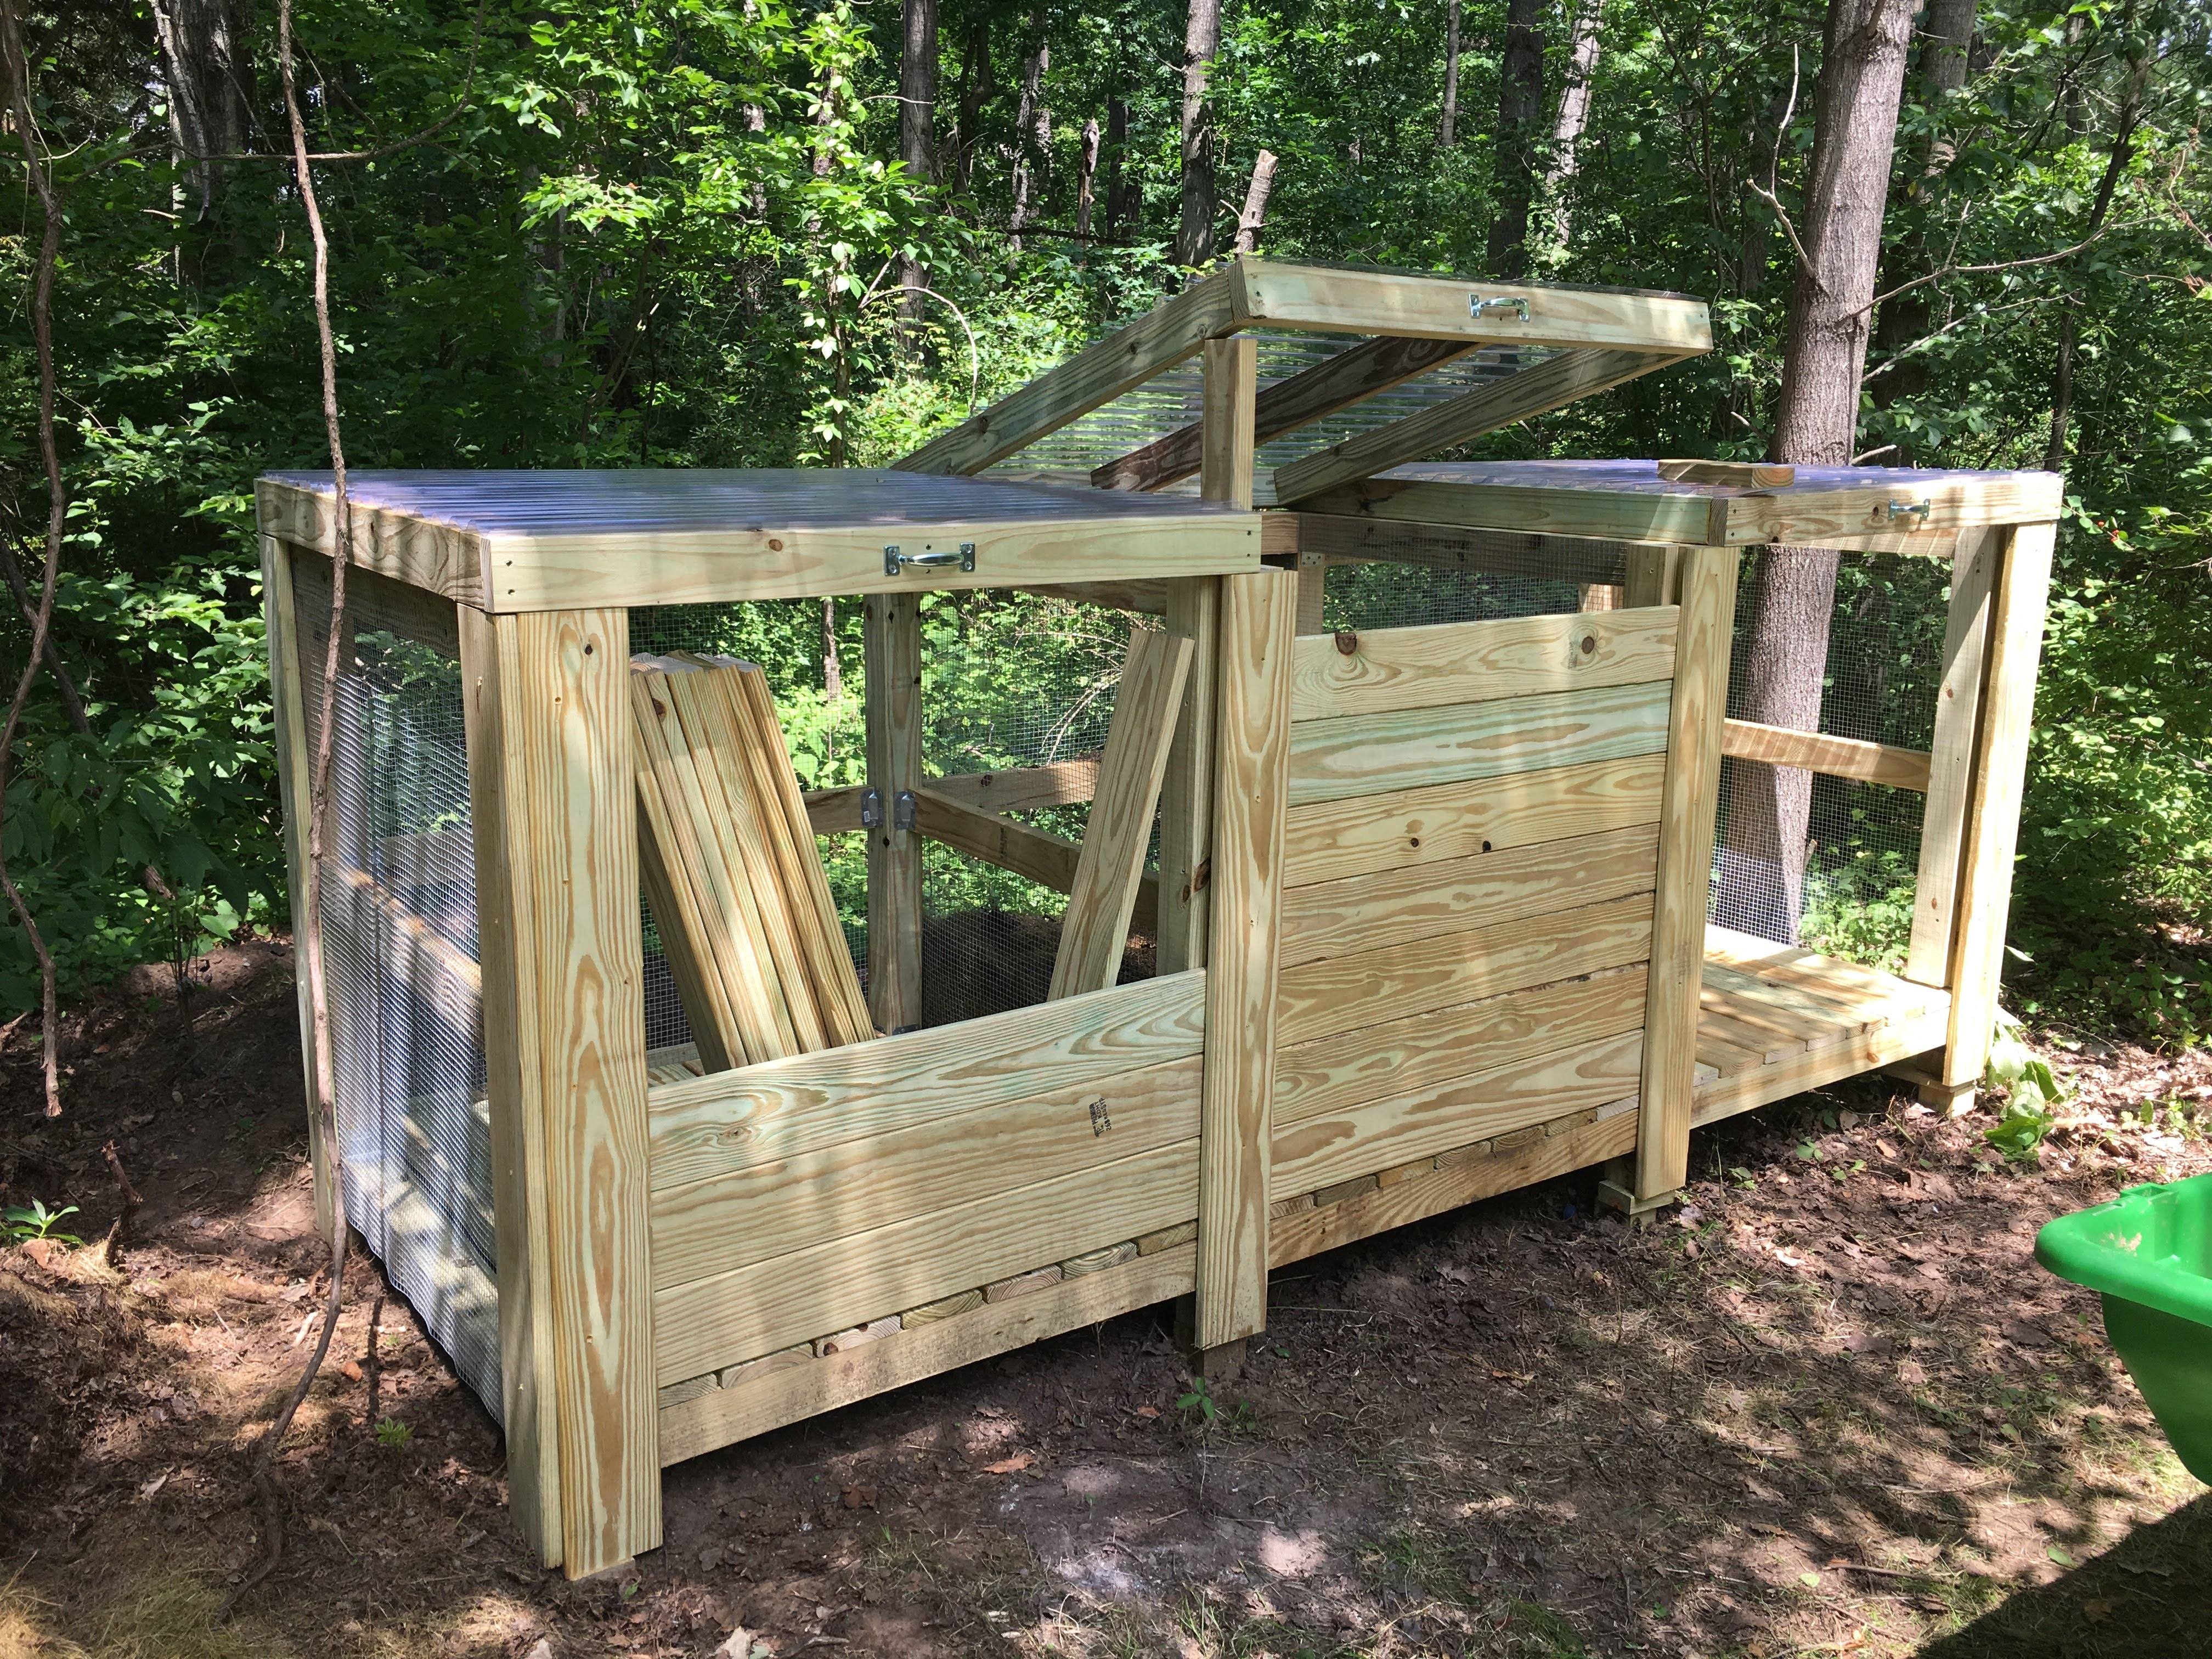
\includegraphics[width=.65\textwidth]{images/actual_finished.JPG}}


\begin{document}

\begin{frame}
\titlepage % Print the title page as the first slide
\end{frame}

\begin{frame}
\frametitle{Overview} % Table of contents slide, comment this block out to remove it
\tableofcontents % Throughout your presentation, if you choose to use \section{} and \subsection{} commands, these will automatically be printed on this slide as an overview of your presentation
\end{frame}

%----------------------------------------------------------------------------------------
%	PRESENTATION SLIDES
%----------------------------------------------------------------------------------------

\section{Design Overview}

\begin{frame}
  \frametitle{Major Features}
  \begin{itemize}
    \item Three bin layout, standard for compost management
    \item Modular design, can be built in parts and raised in another location
    \item Removable front sleeves allow filling of entire bin yet easy access for turnover
    \item Presented design uses treated pine, acknowledging limit then on compost use for edible gardening
  \end{itemize}
\end{frame}

\begin{frame}
  \frametitle{3D View}
  \begin{center}
  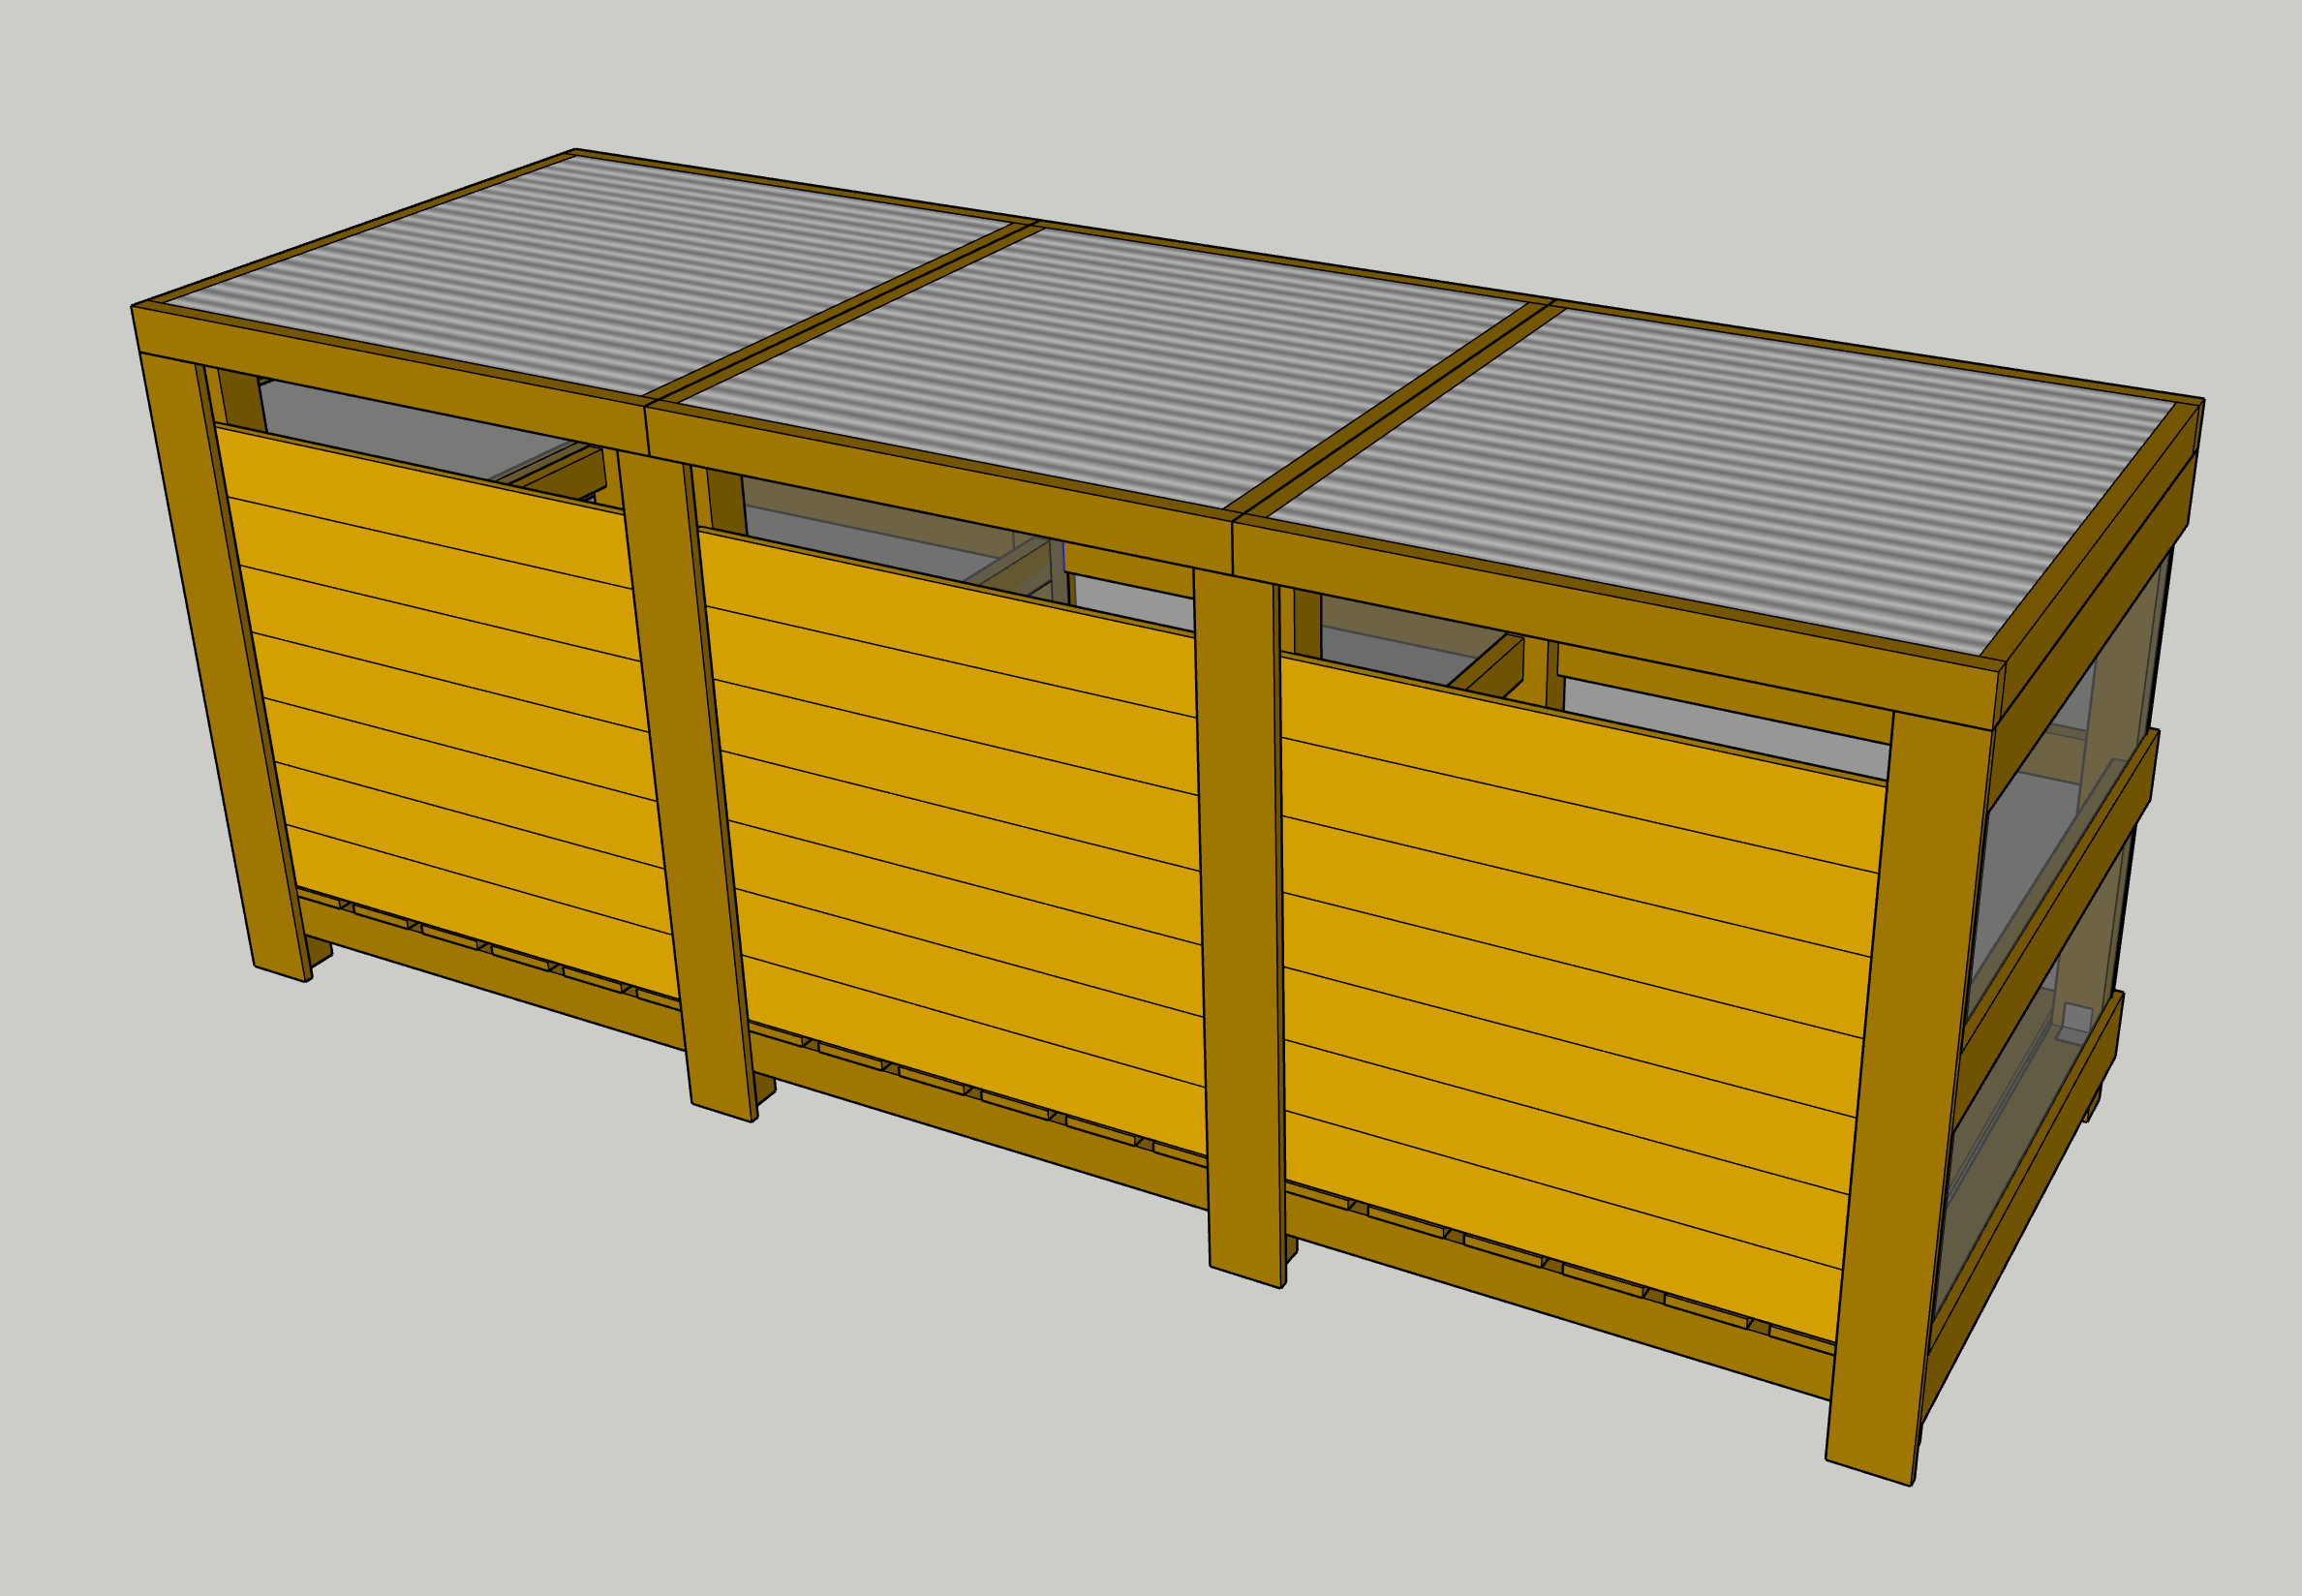
\includegraphics[width=.85\textwidth]{images/FrontPanels.png}
  \end{center}
\end{frame}

\section{Construction}

\begin{frame}
  \frametitle{Approach}
  \begin{enumerate}
  \item Build 4 x upright frames, 1 for each end and 2 in the middle
  \item Build two side cubes in location (\emph{I built standing on its front, and then when skeleton structure finished I flipped it up to sit on blocks on ground})
  \item Join two side cubes with spreaders (\emph{Then flip up so standing upright in location})
  \item Install floors and struts
  \item Install sleeve guides, cut sleeves to length
  \item Install lids
  \end{enumerate}
\end{frame}

\begin{frame}
  \frametitle{Left/Right Cube Construction}
  \begin{itemize}
  \item Approx 4' x 4' overall cube size, 4''x4'' treated pine
  \item 4''x4'' lengths for outside of cube, 2''x4'' for mid-spacers
  \item 90 degree angle metal brackets, 8 total screws each---simpler construction as no jointing
  \item Next page shows dimensions
  \end{itemize}
\end{frame}

\begin{frame}
  \frametitle{Left/Right Cube View}
  \begin{center}
  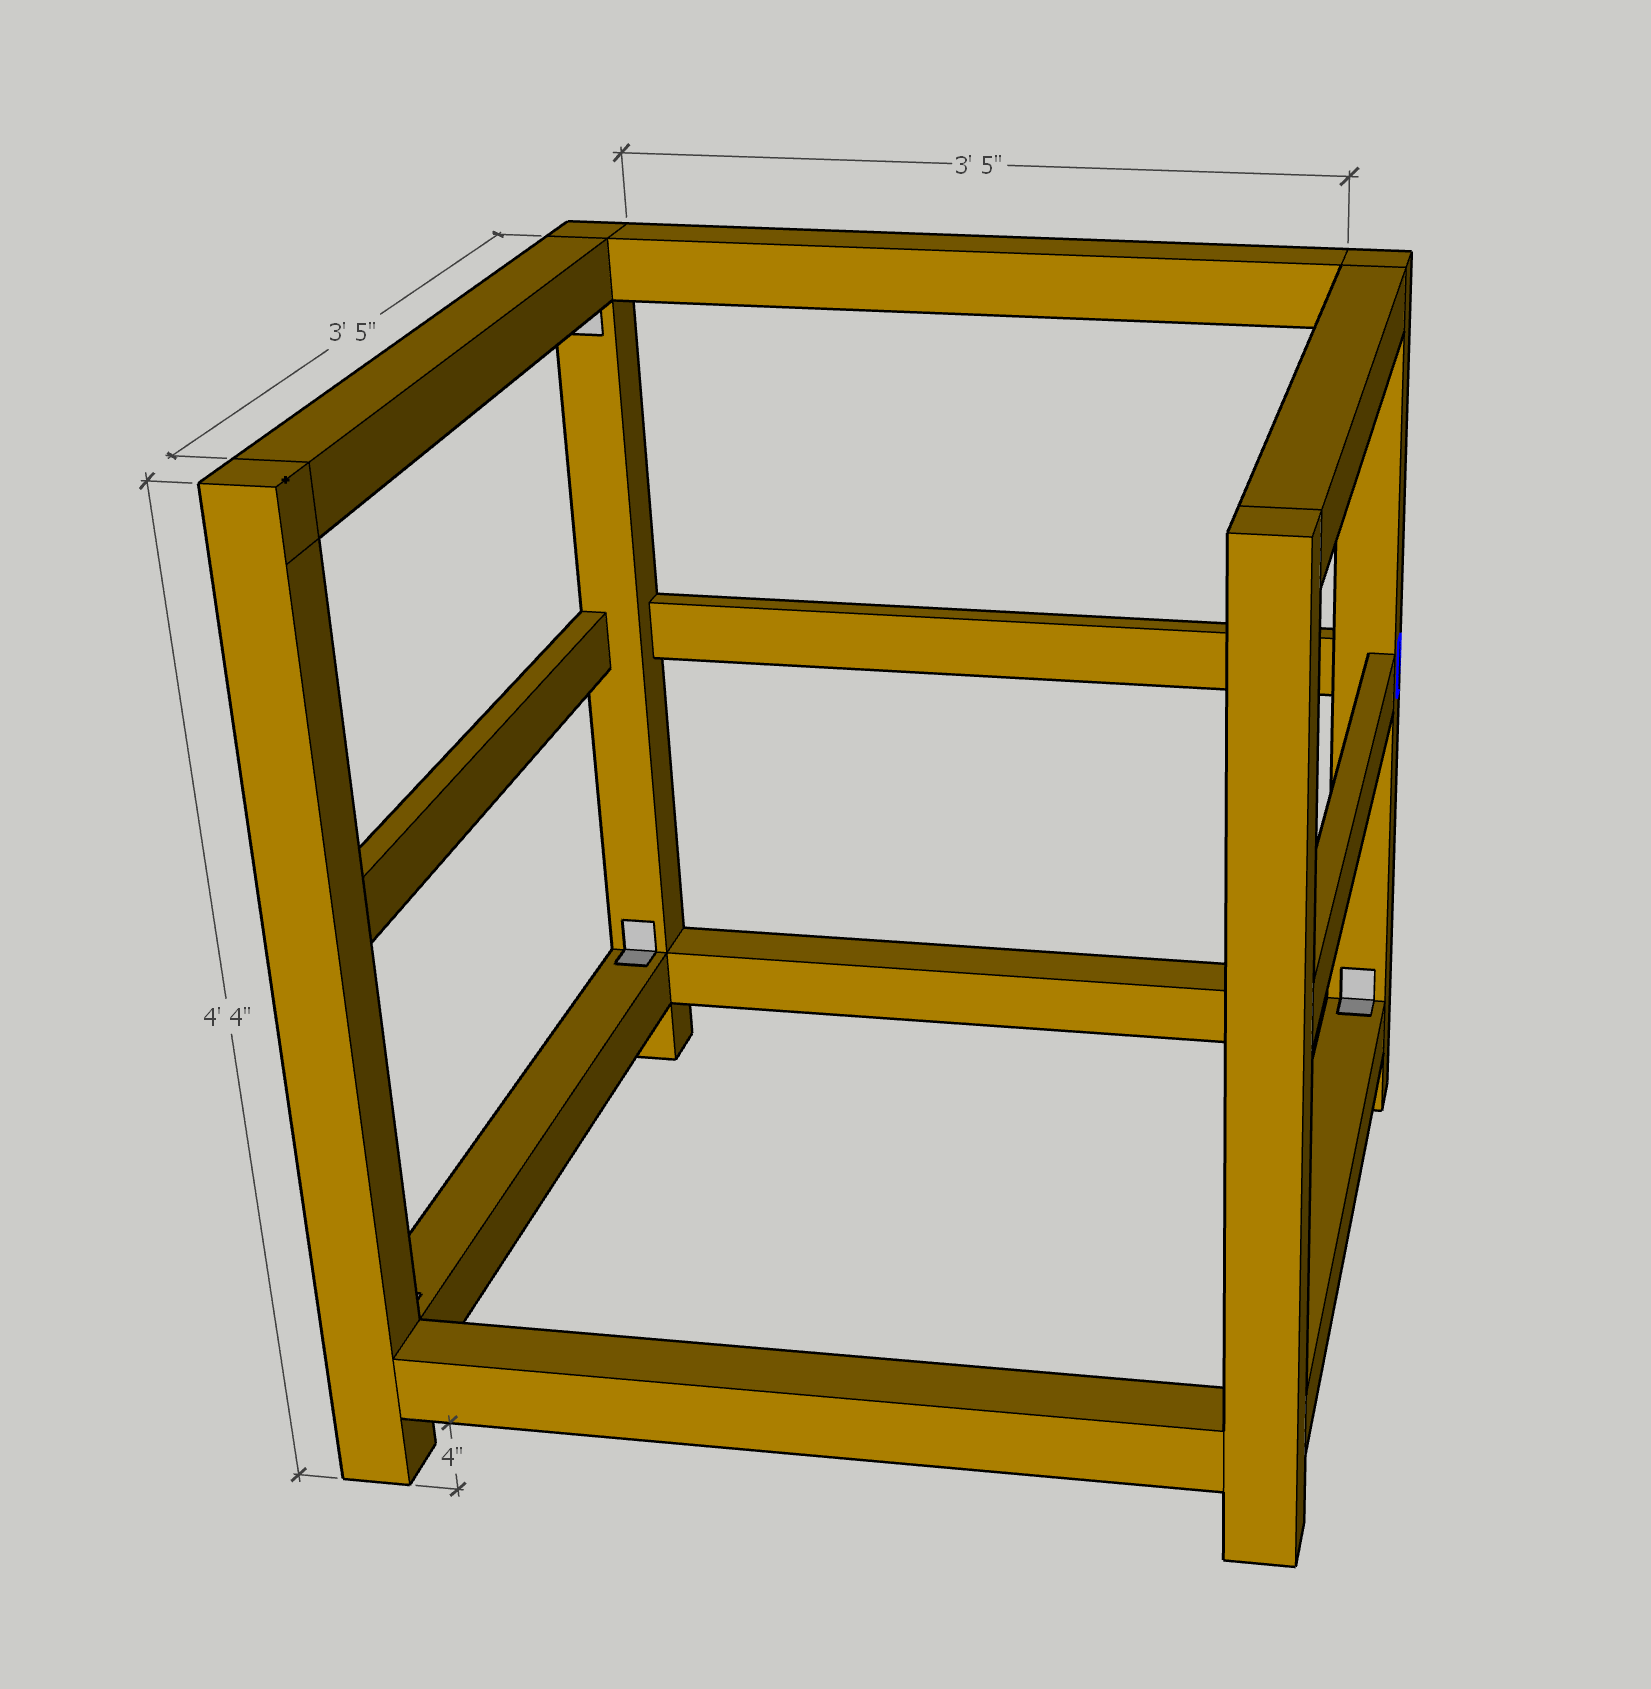
\includegraphics[width=0.5\textwidth]{images/SideCubeFull.png}
  \end{center}
\end{frame}

\begin{frame}
  \frametitle{Full Cube Skeleton}
  \begin{itemize}
  \item As noted in Approach, recommend building the skeleton on its front and then flip up into place on blocks
  \item Connect the cubes with spreaders of same 3'5'' length
    \item Once flipped up, recommend installing the 45 degree struts at far corners of the side cubes (this helps limit the sides falling outward)
  \end{itemize}
\end{frame}

\begin{frame}
  \frametitle{Full Cube Skeleton View}
  \begin{center}
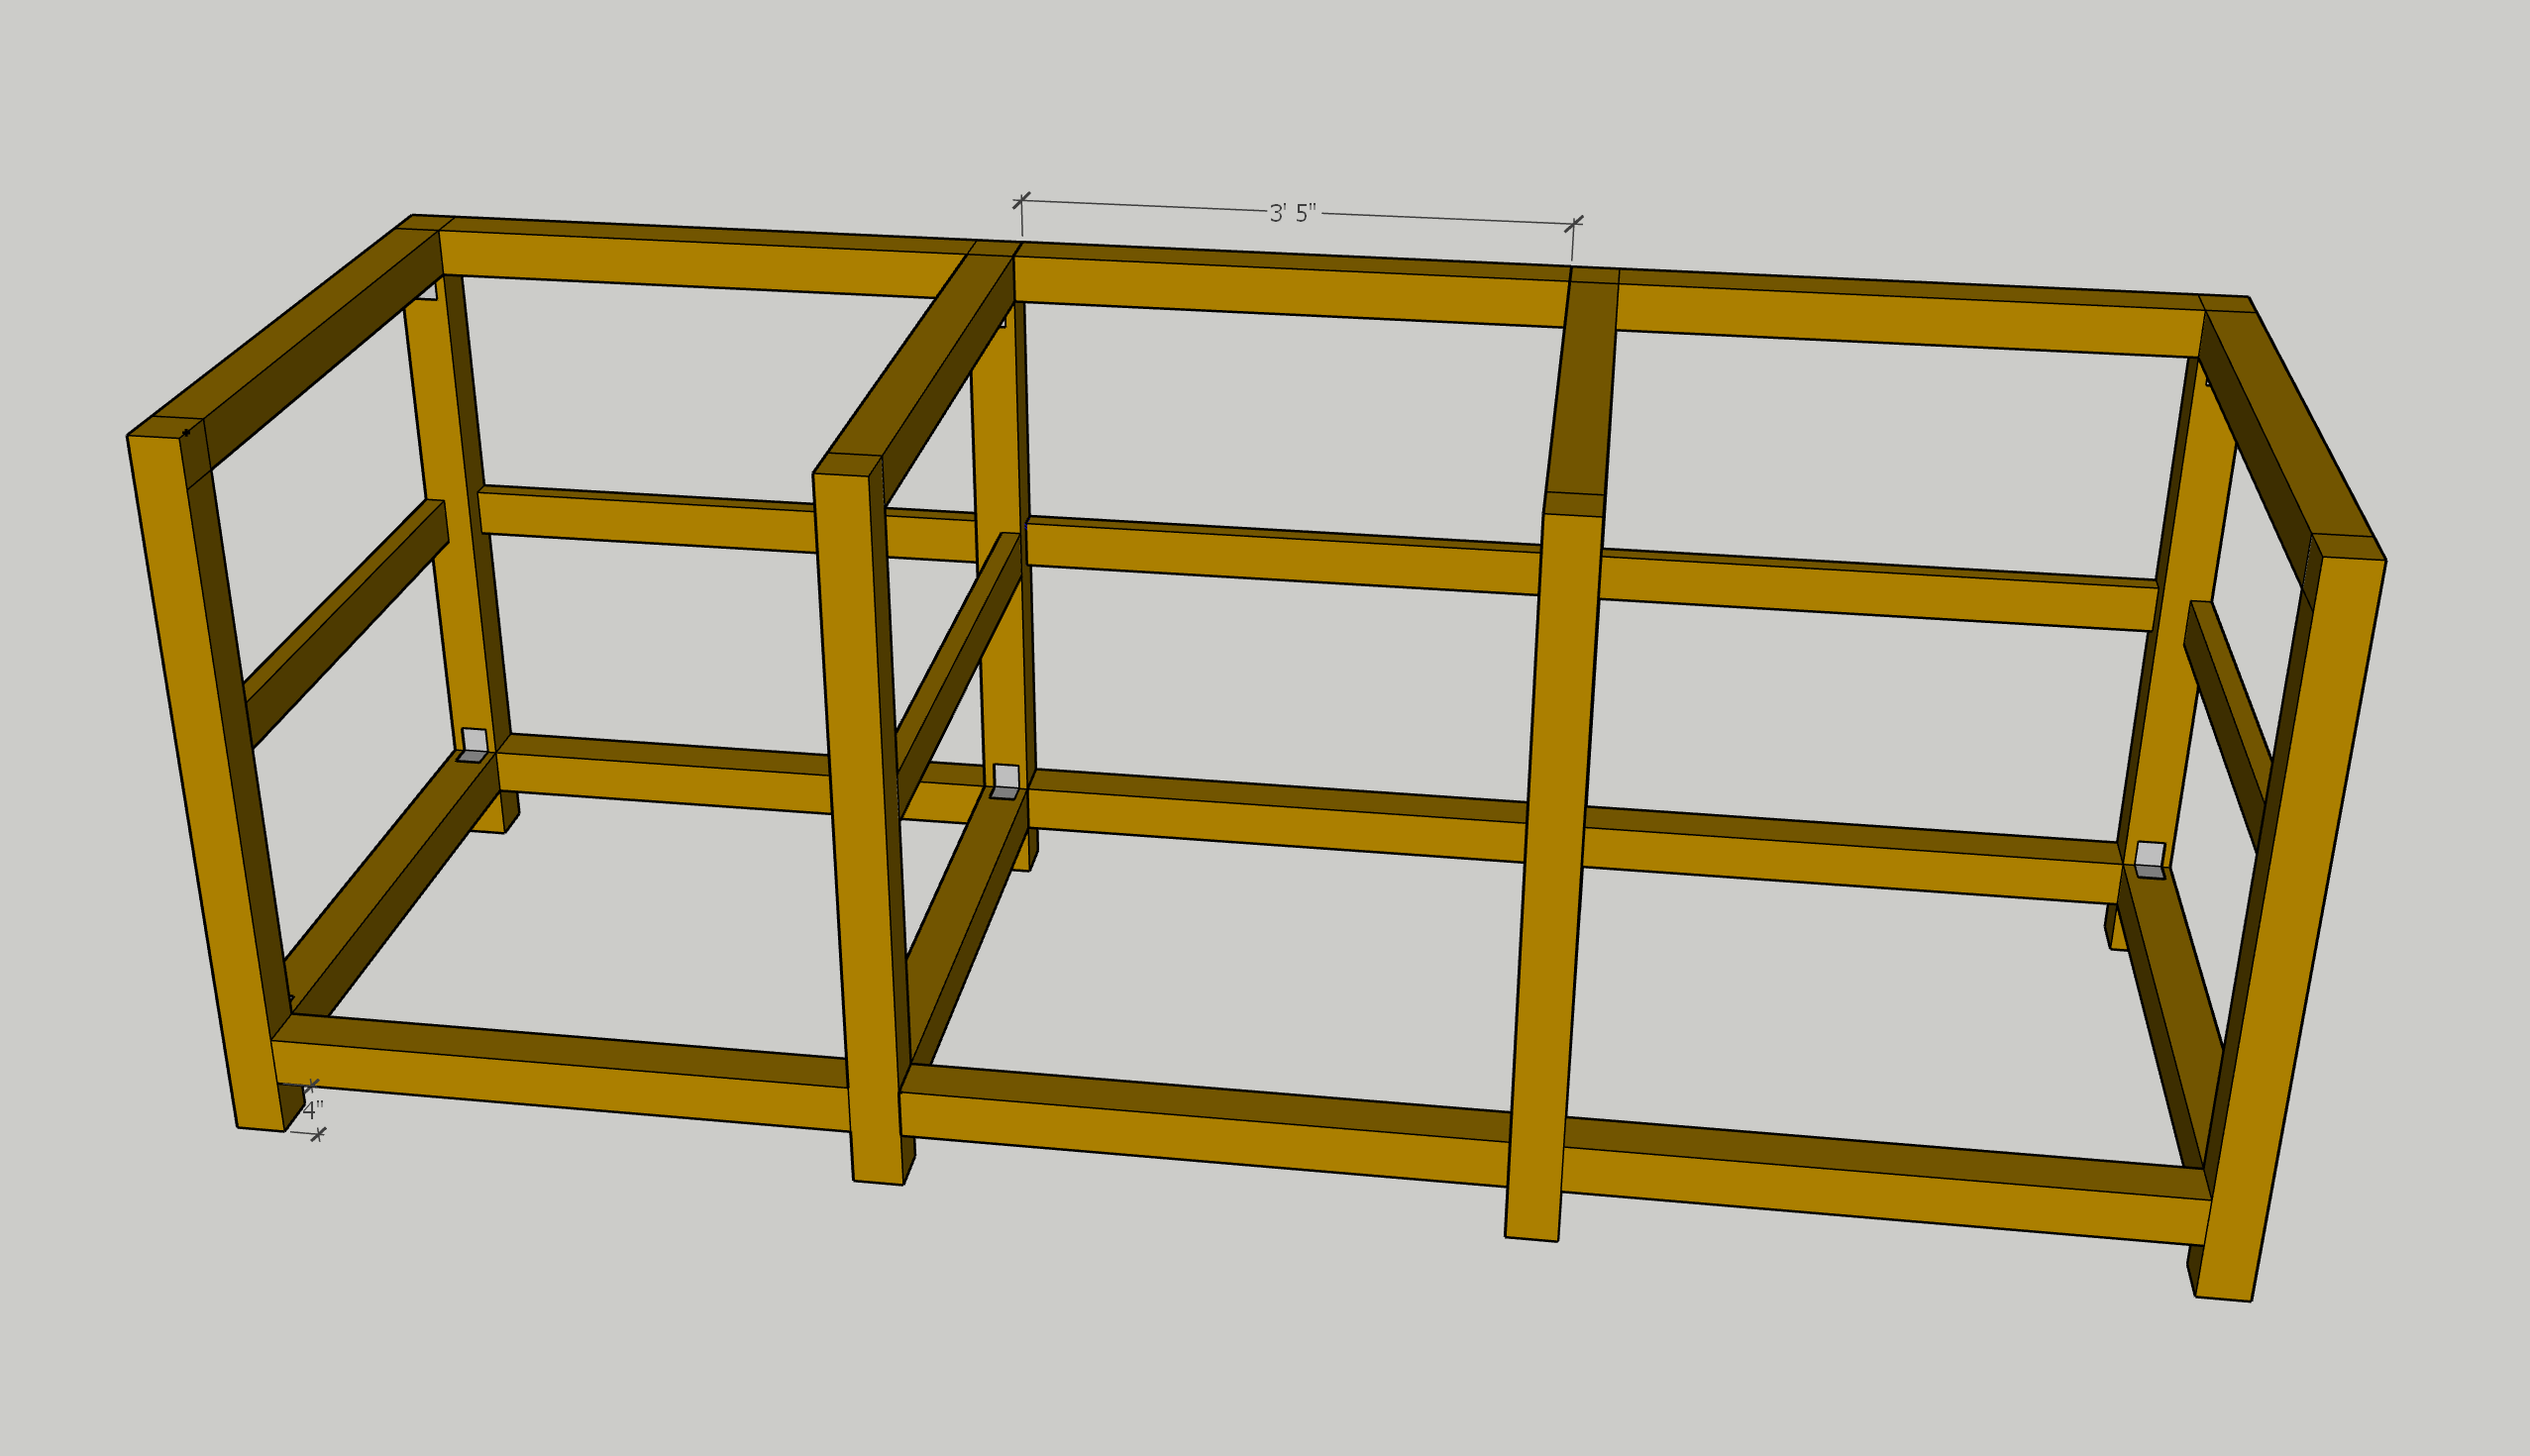
\includegraphics[width=0.85\textwidth]{images/FullCubes.png}
  \end{center}
\end{frame}

\begin{frame}
  \frametitle{Struts}
 \begin{center}
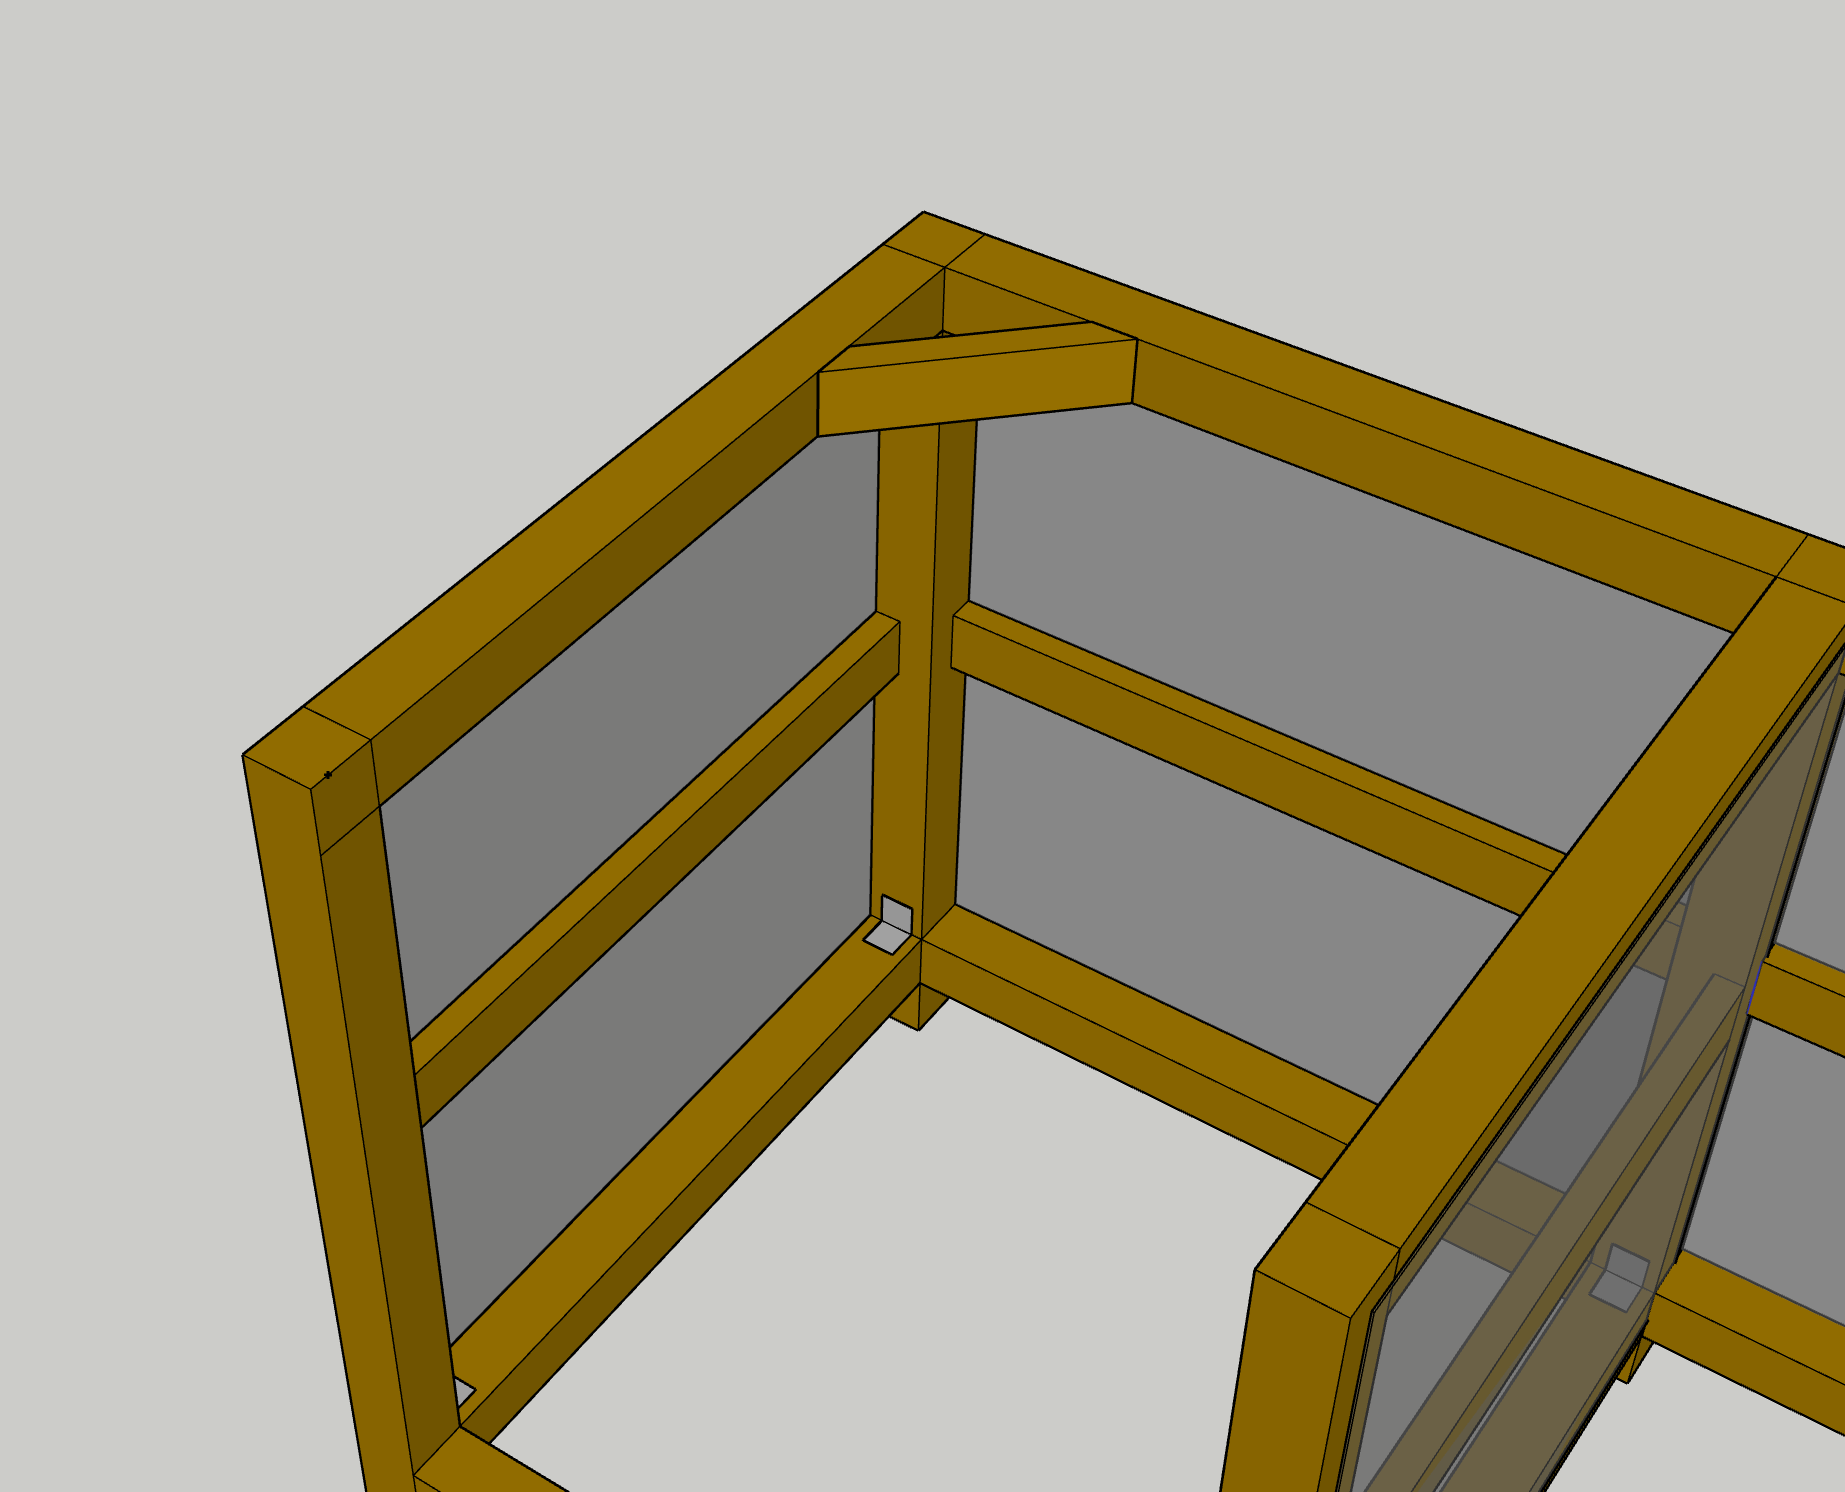
\includegraphics[width=.7\textwidth]{images/Struts.PNG}
 \end{center} 
\end{frame}

\begin{frame}
  \frametitle{Installing Floors}
  \begin{itemize}
  \item 6 lengths each cube, 5/4''x6'' pressure treated pine
  \item Measure and cut to fit front to back of cube (at front, the lowest sleeve then sits on the flooring)
    \item Install with 2 screws either end
  \item Actual image shows full cube skeleton with one floor installed---flow in these instructions has grids installed after floors but in actual build I installed grids before floors, not that it matters
  \end{itemize}
\end{frame}

\begin{frame}
  \frametitle{3D Floors View}
  \begin{center}
    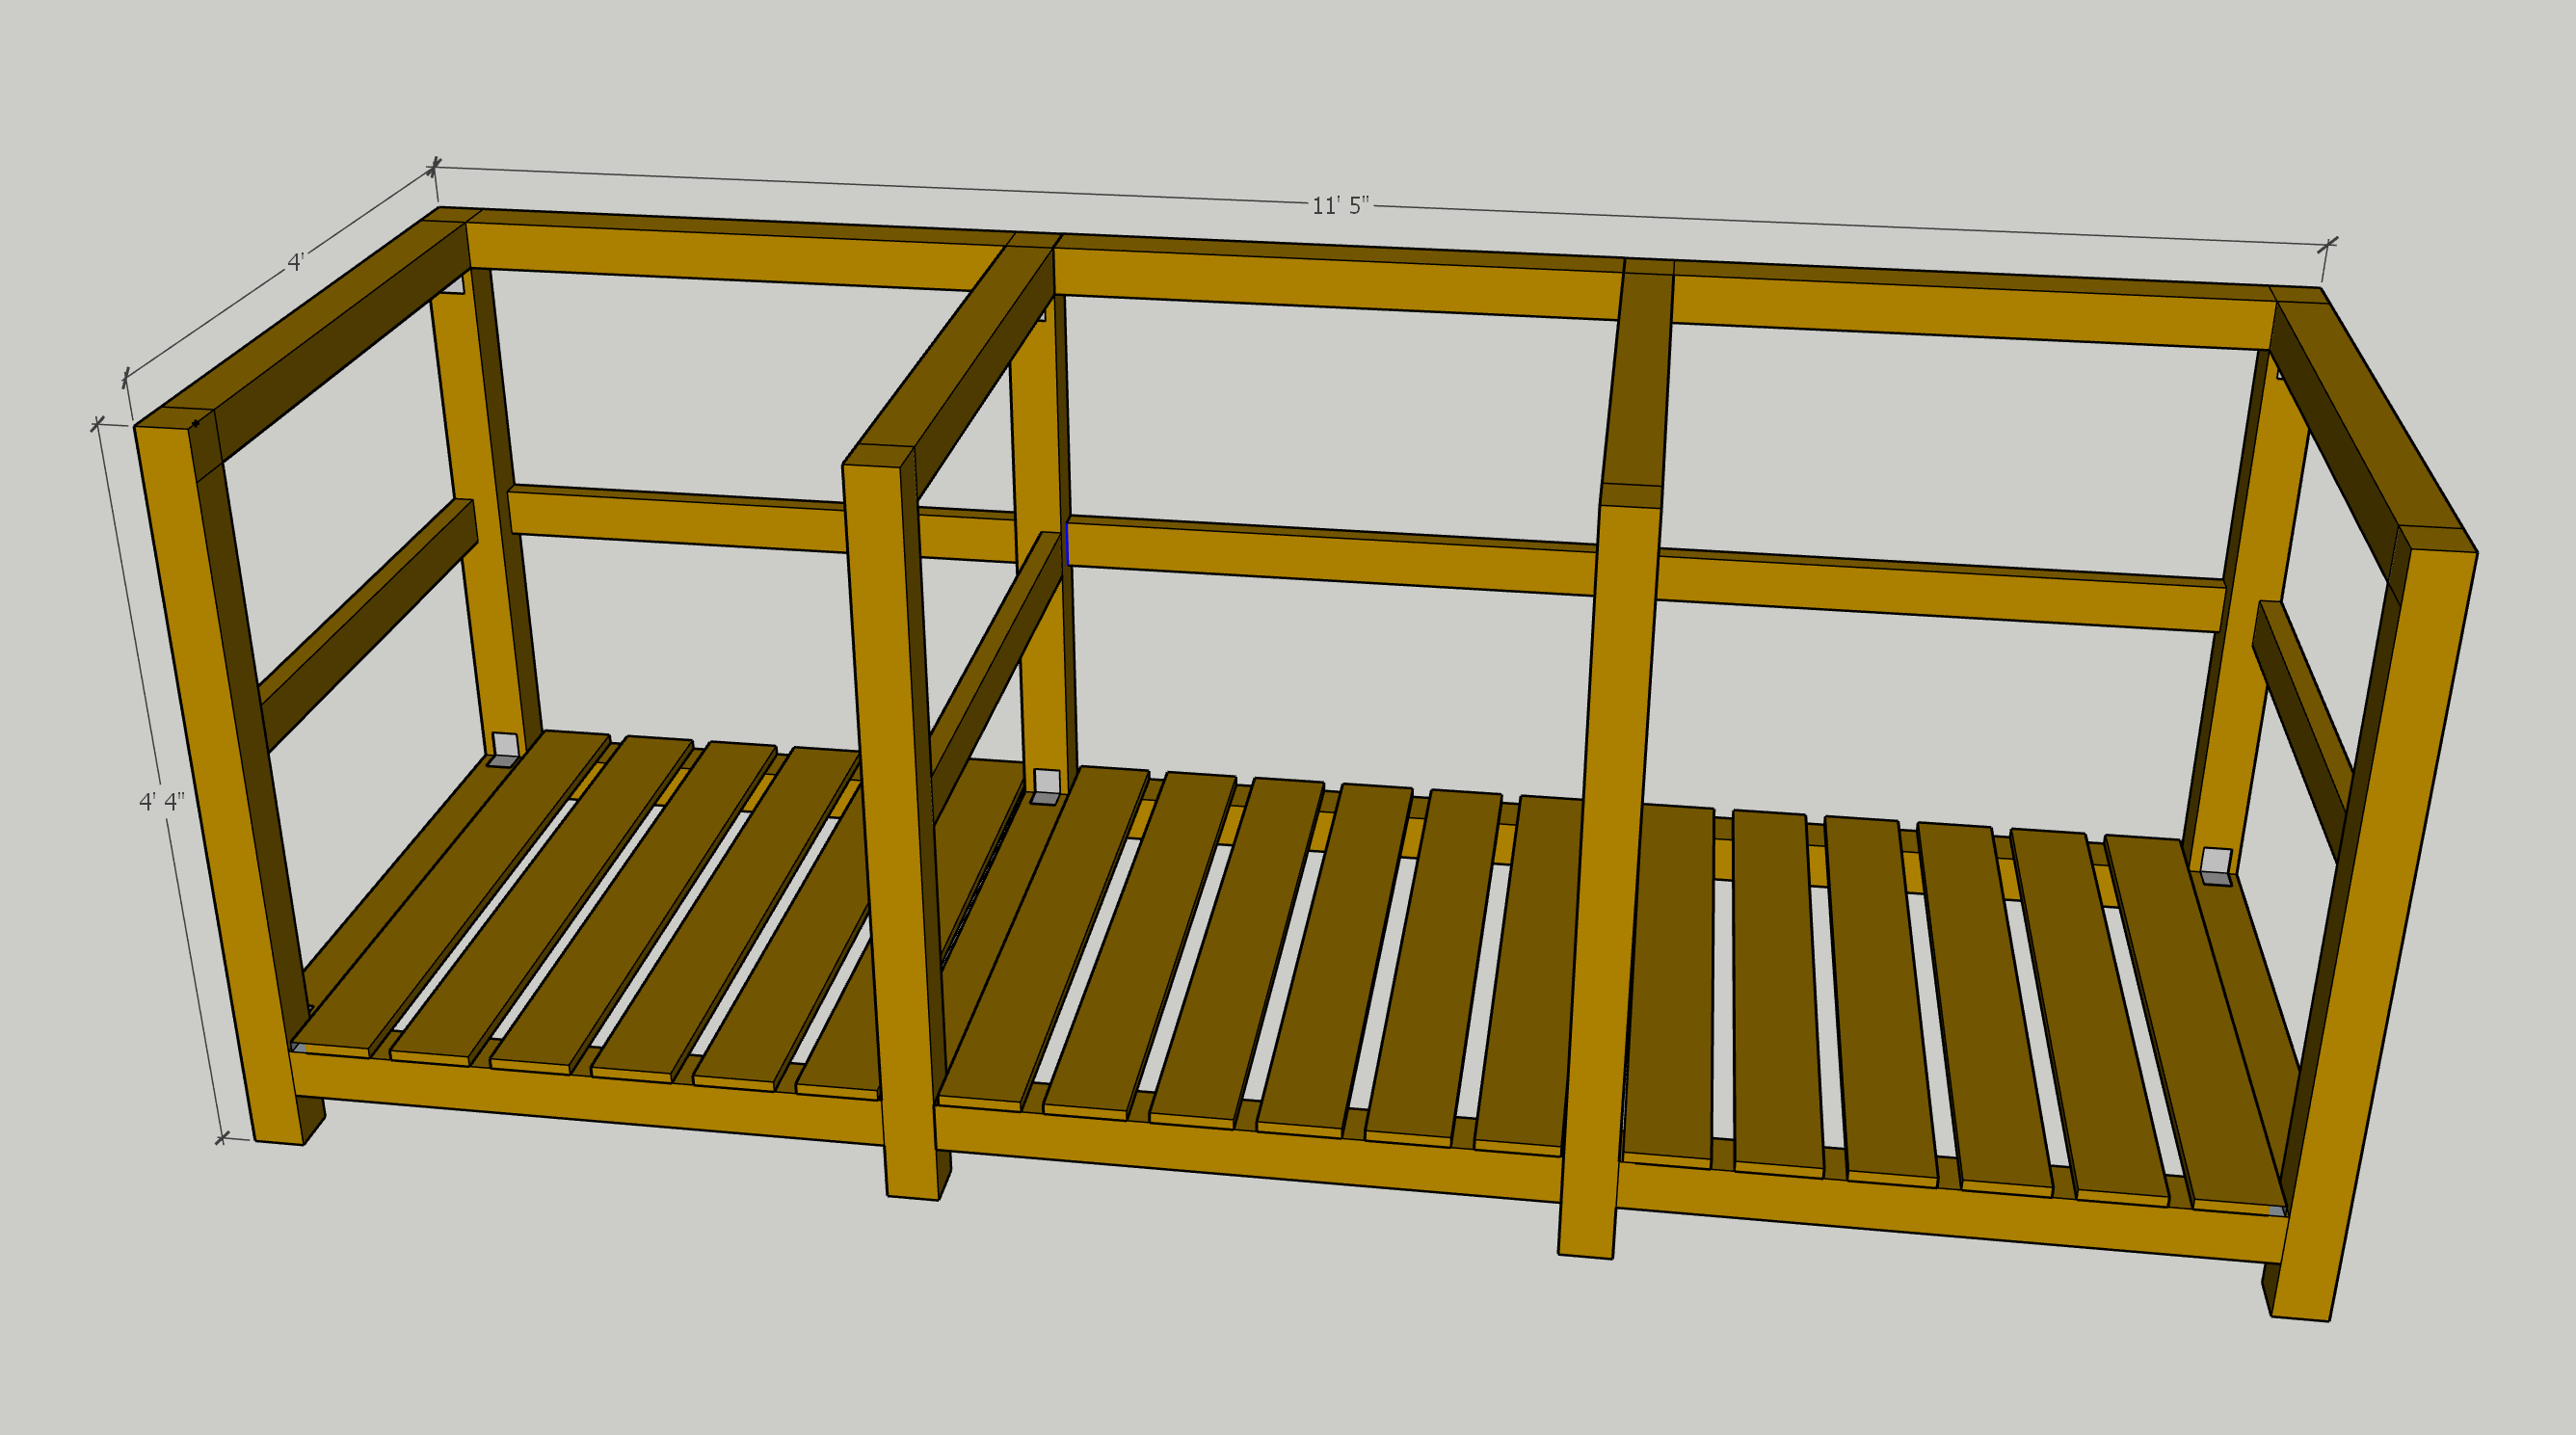
\includegraphics[width=0.85\textwidth]{images/FullCubesWFloor.png}
  \end{center}
\end{frame}

\begin{frame}
  \frametitle{Actual Partial Build}
  \begin{center}
      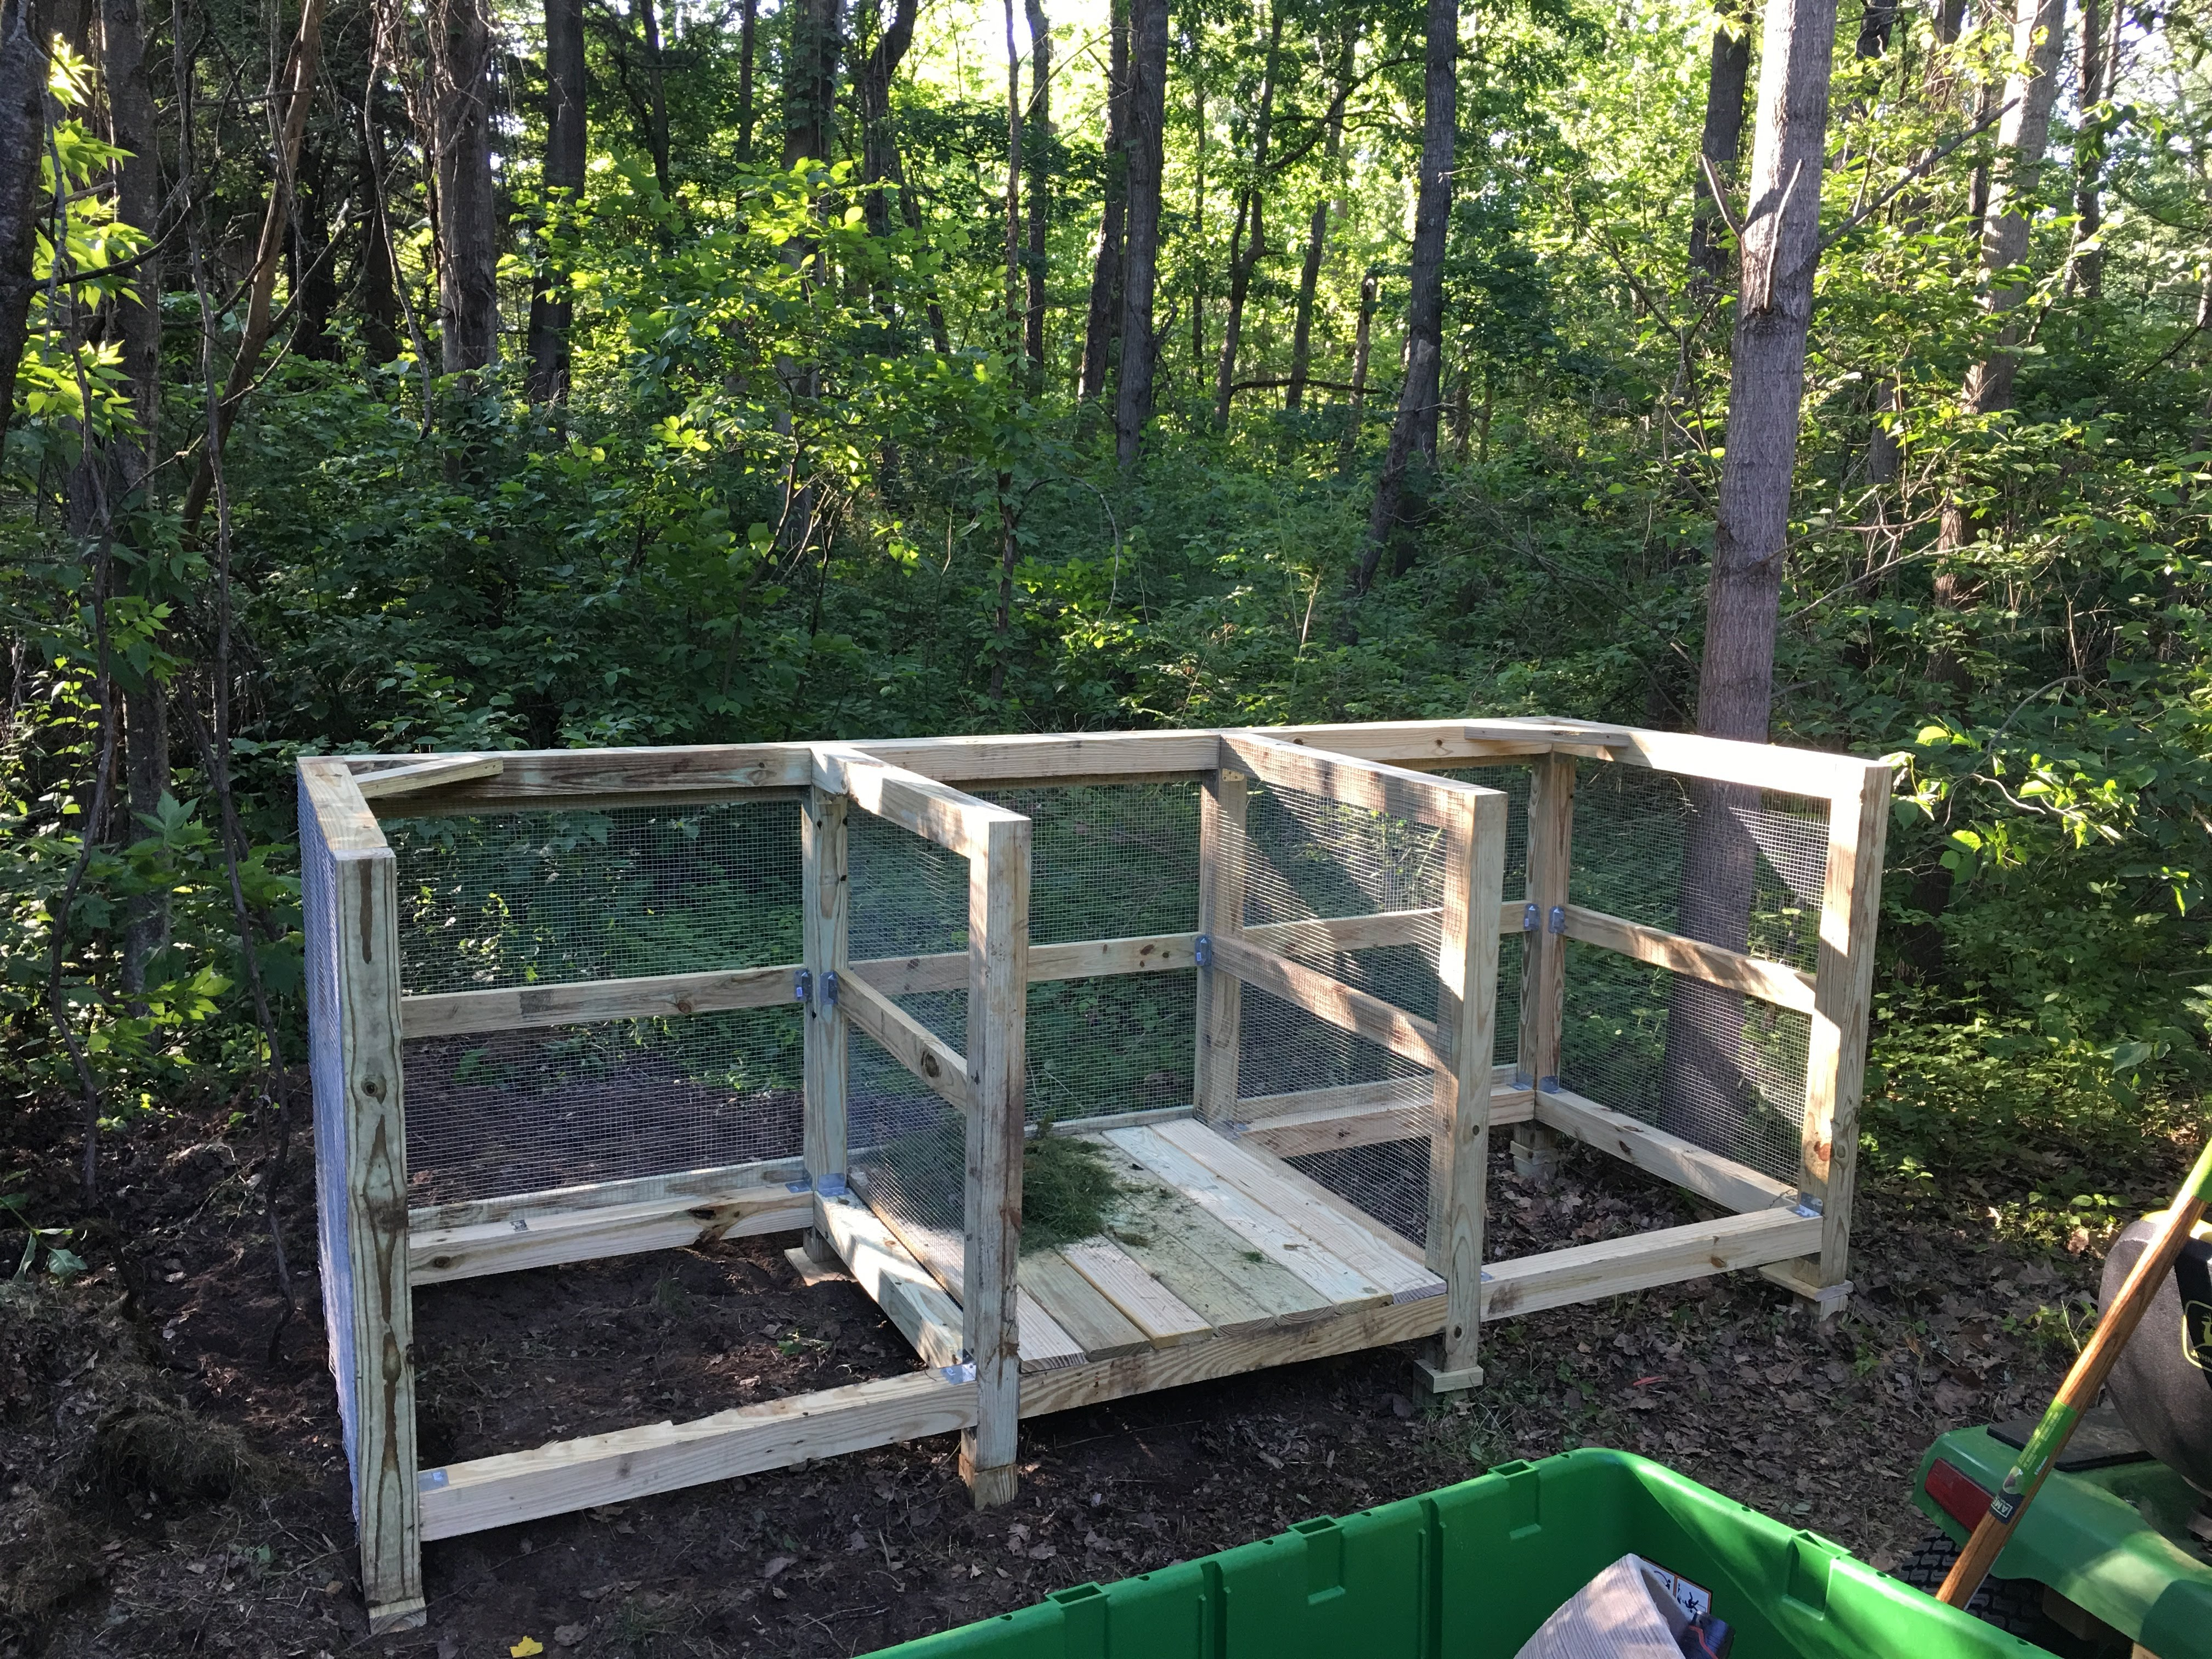
\includegraphics[width=0.75\textwidth]{images/actual_partial.JPG}
  \end{center}
\end{frame}

\begin{frame}
  \frametitle{Install Front Panels \& Sleeve Guides}
  \begin{itemize}
  \item From 5/4''x6'' lengths install full height panels, flush with sides on far left/right frames, centered on two middle ones---these act as the front guide for the removable sleeves
  \item Install with 4 to 5 screws up the vertical
  \item Install 2''x4'' sleeve guides behind, measure and cut above floor (\emph{no need to be flush, I have about 1'' spacing})
  \item Trick on the sleeve guides is to have some of the front sleeve panels cut already and use those to ensure sufficient spacing---I screwed back sleeve in at top first with one temporary screw and adjusted until found good fit
    \item Watch for variations in the front sleeve depth, they will also expand/contract with humidity and temperature
  \end{itemize}
\end{frame}

\begin{frame}
  \frametitle{Front Panels 3D View}
  \begin{center}
  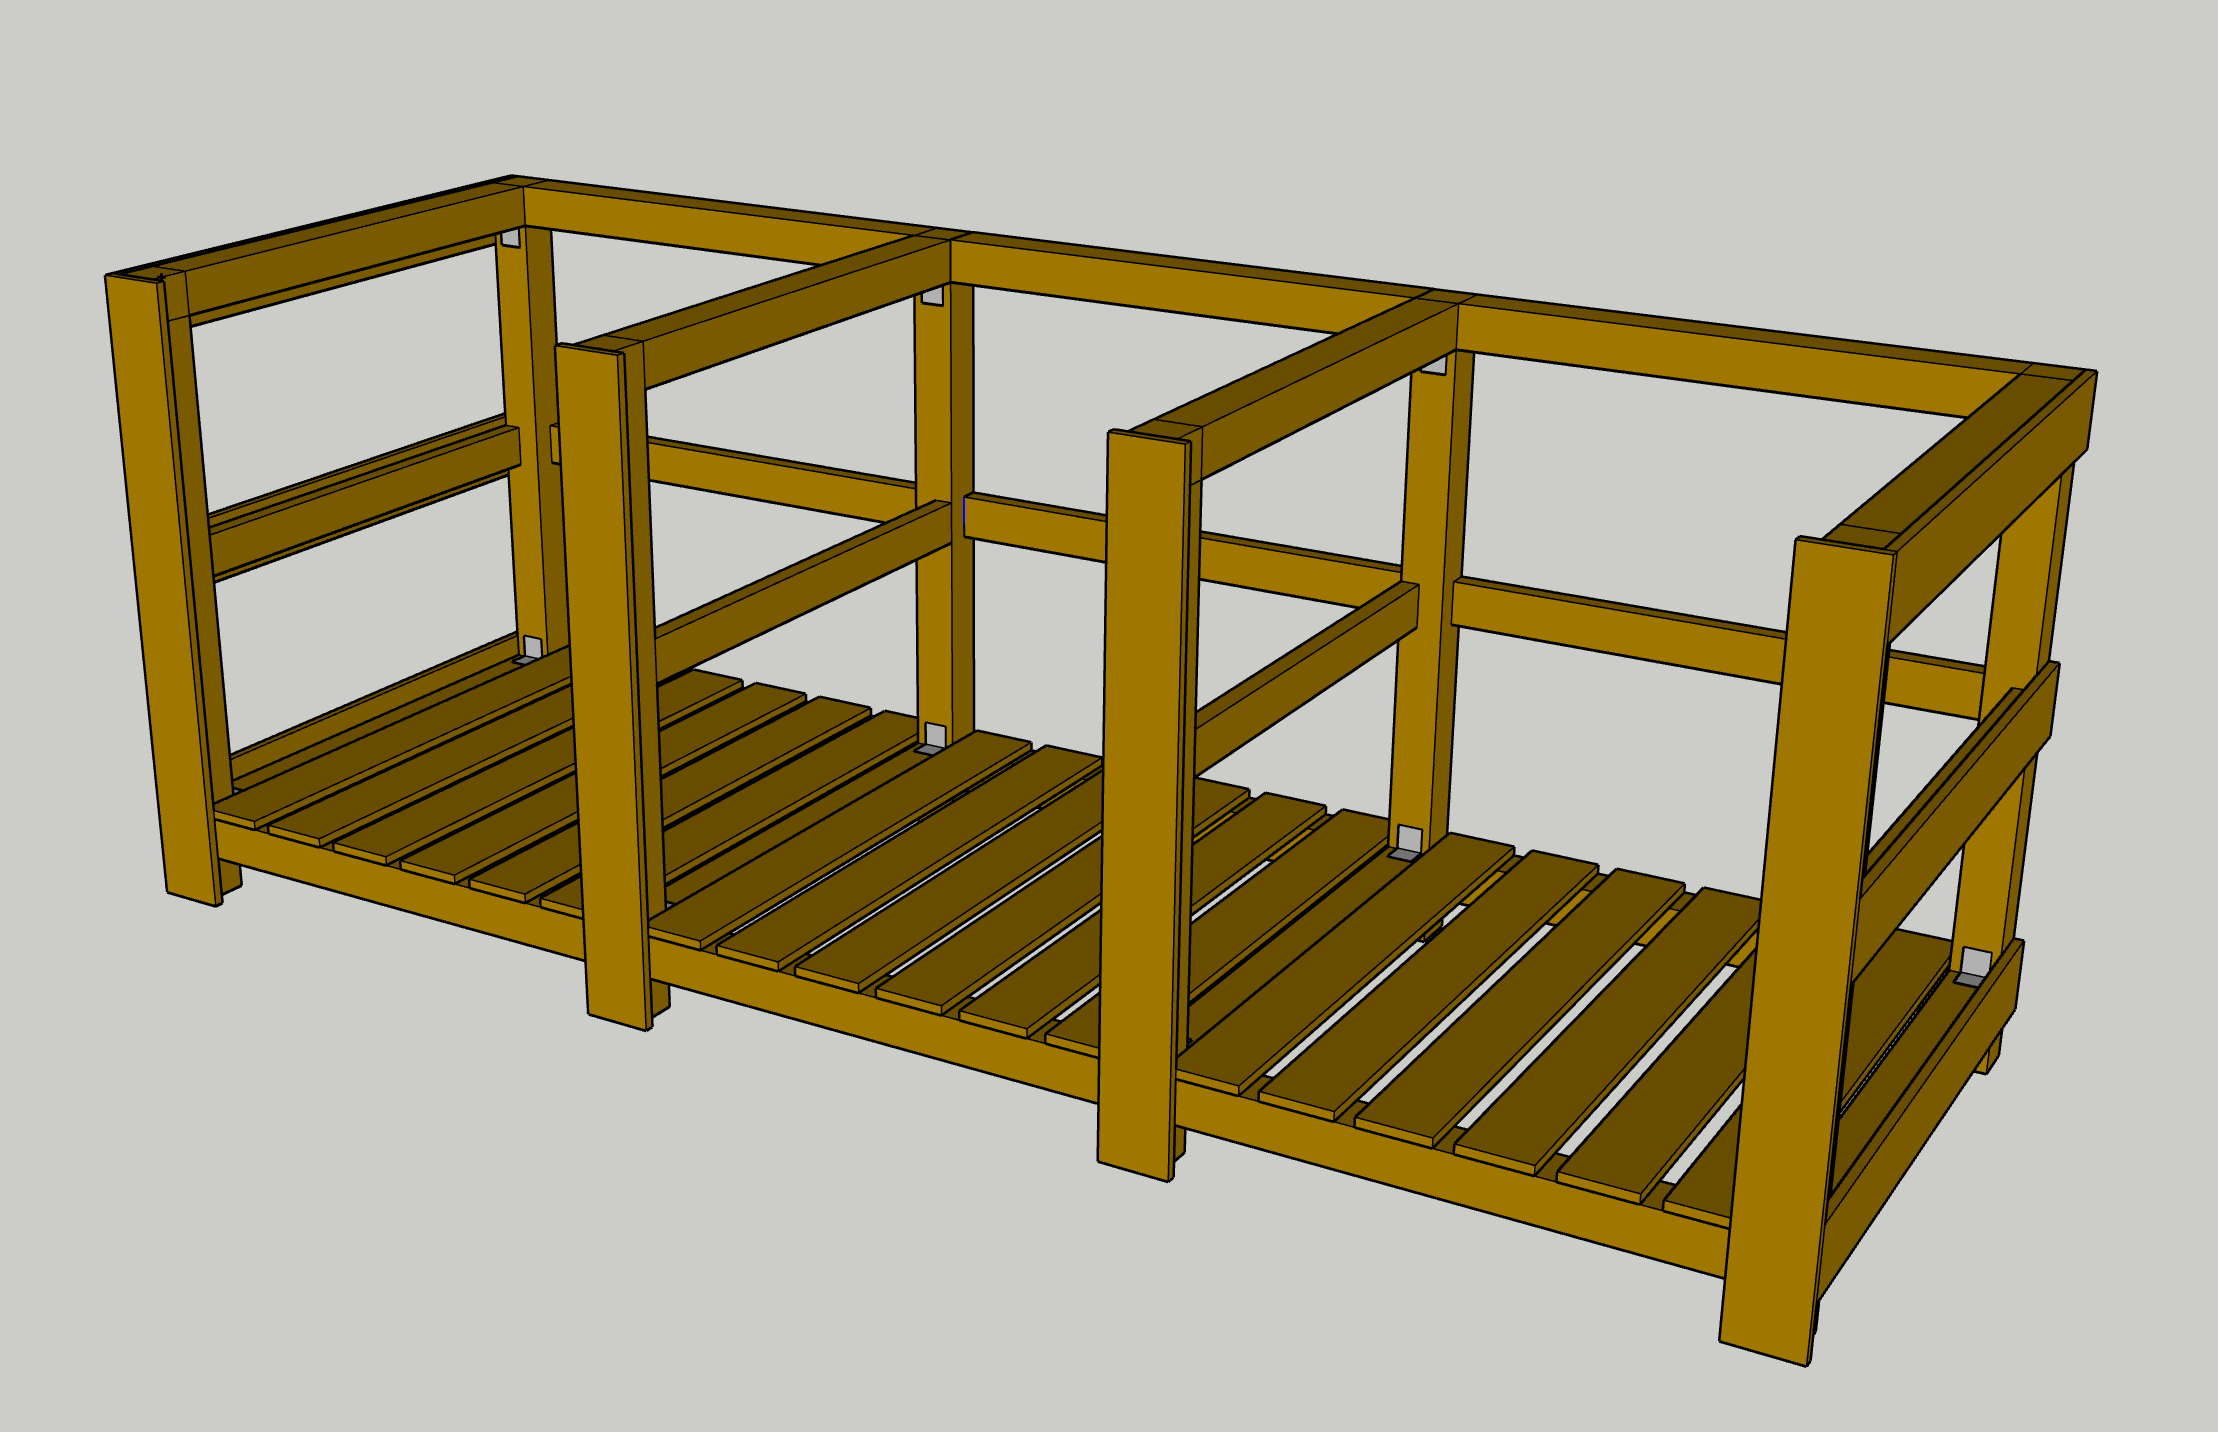
\includegraphics[width=0.85\textwidth]{images/CubesWPaneling.png}  
  \end{center}
\end{frame}

\begin{frame}
  \frametitle{Sleeve Guides 3D View}
  \begin{center}
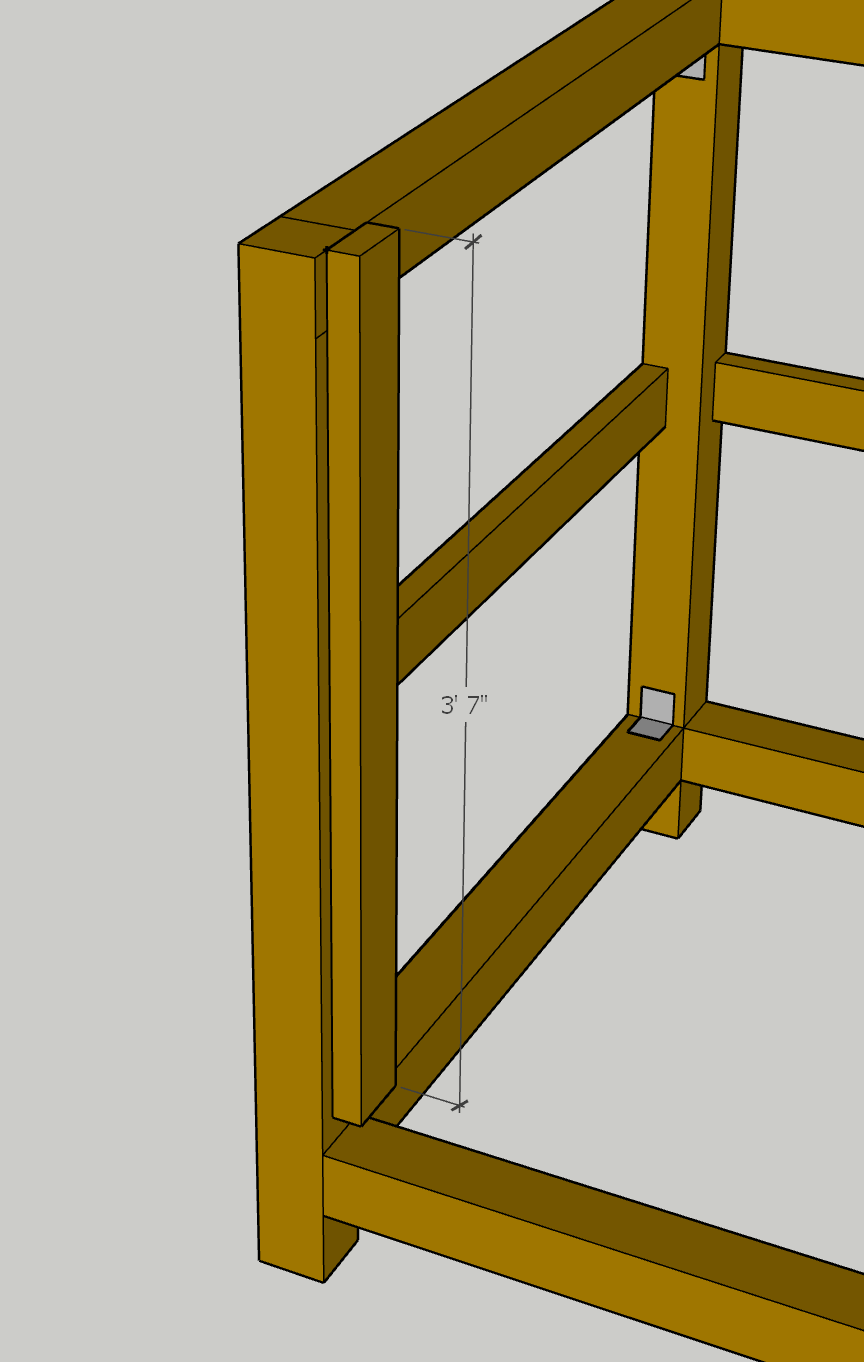
\includegraphics[width=.35\textwidth]{images/Sleeves.png}
  \end{center}
\end{frame}

\begin{frame}
  \frametitle{Lids \& Completion}
  \begin{itemize}
  \item Build lids out of 2''x4'' frames, with one spreader front to back (\emph{I glued the joints for strength and screwed in from butted ends})
    \item Dimensions for lids should be measured in situ, for half/half coverage over internal frames---2x hinges per lid on paneling at back, handle on front
  \item Material for lid cover can be anything, deisgn here has corrugated plastic sheeting, which happened to fit well in two just overlapping layers for each lid
    \item Final step then to finish cutting all the sleeves, unlikely need full set for all three---note though that sleeve lengths may be specific to left/right vs middle cube depending on final dimensions of build (\emph{I have 1/2'' difference and cut sleeves of two lengths})
  \end{itemize}
\end{frame}

\begin{frame}
  \frametitle{Final 3D View}
  \begin{center}
  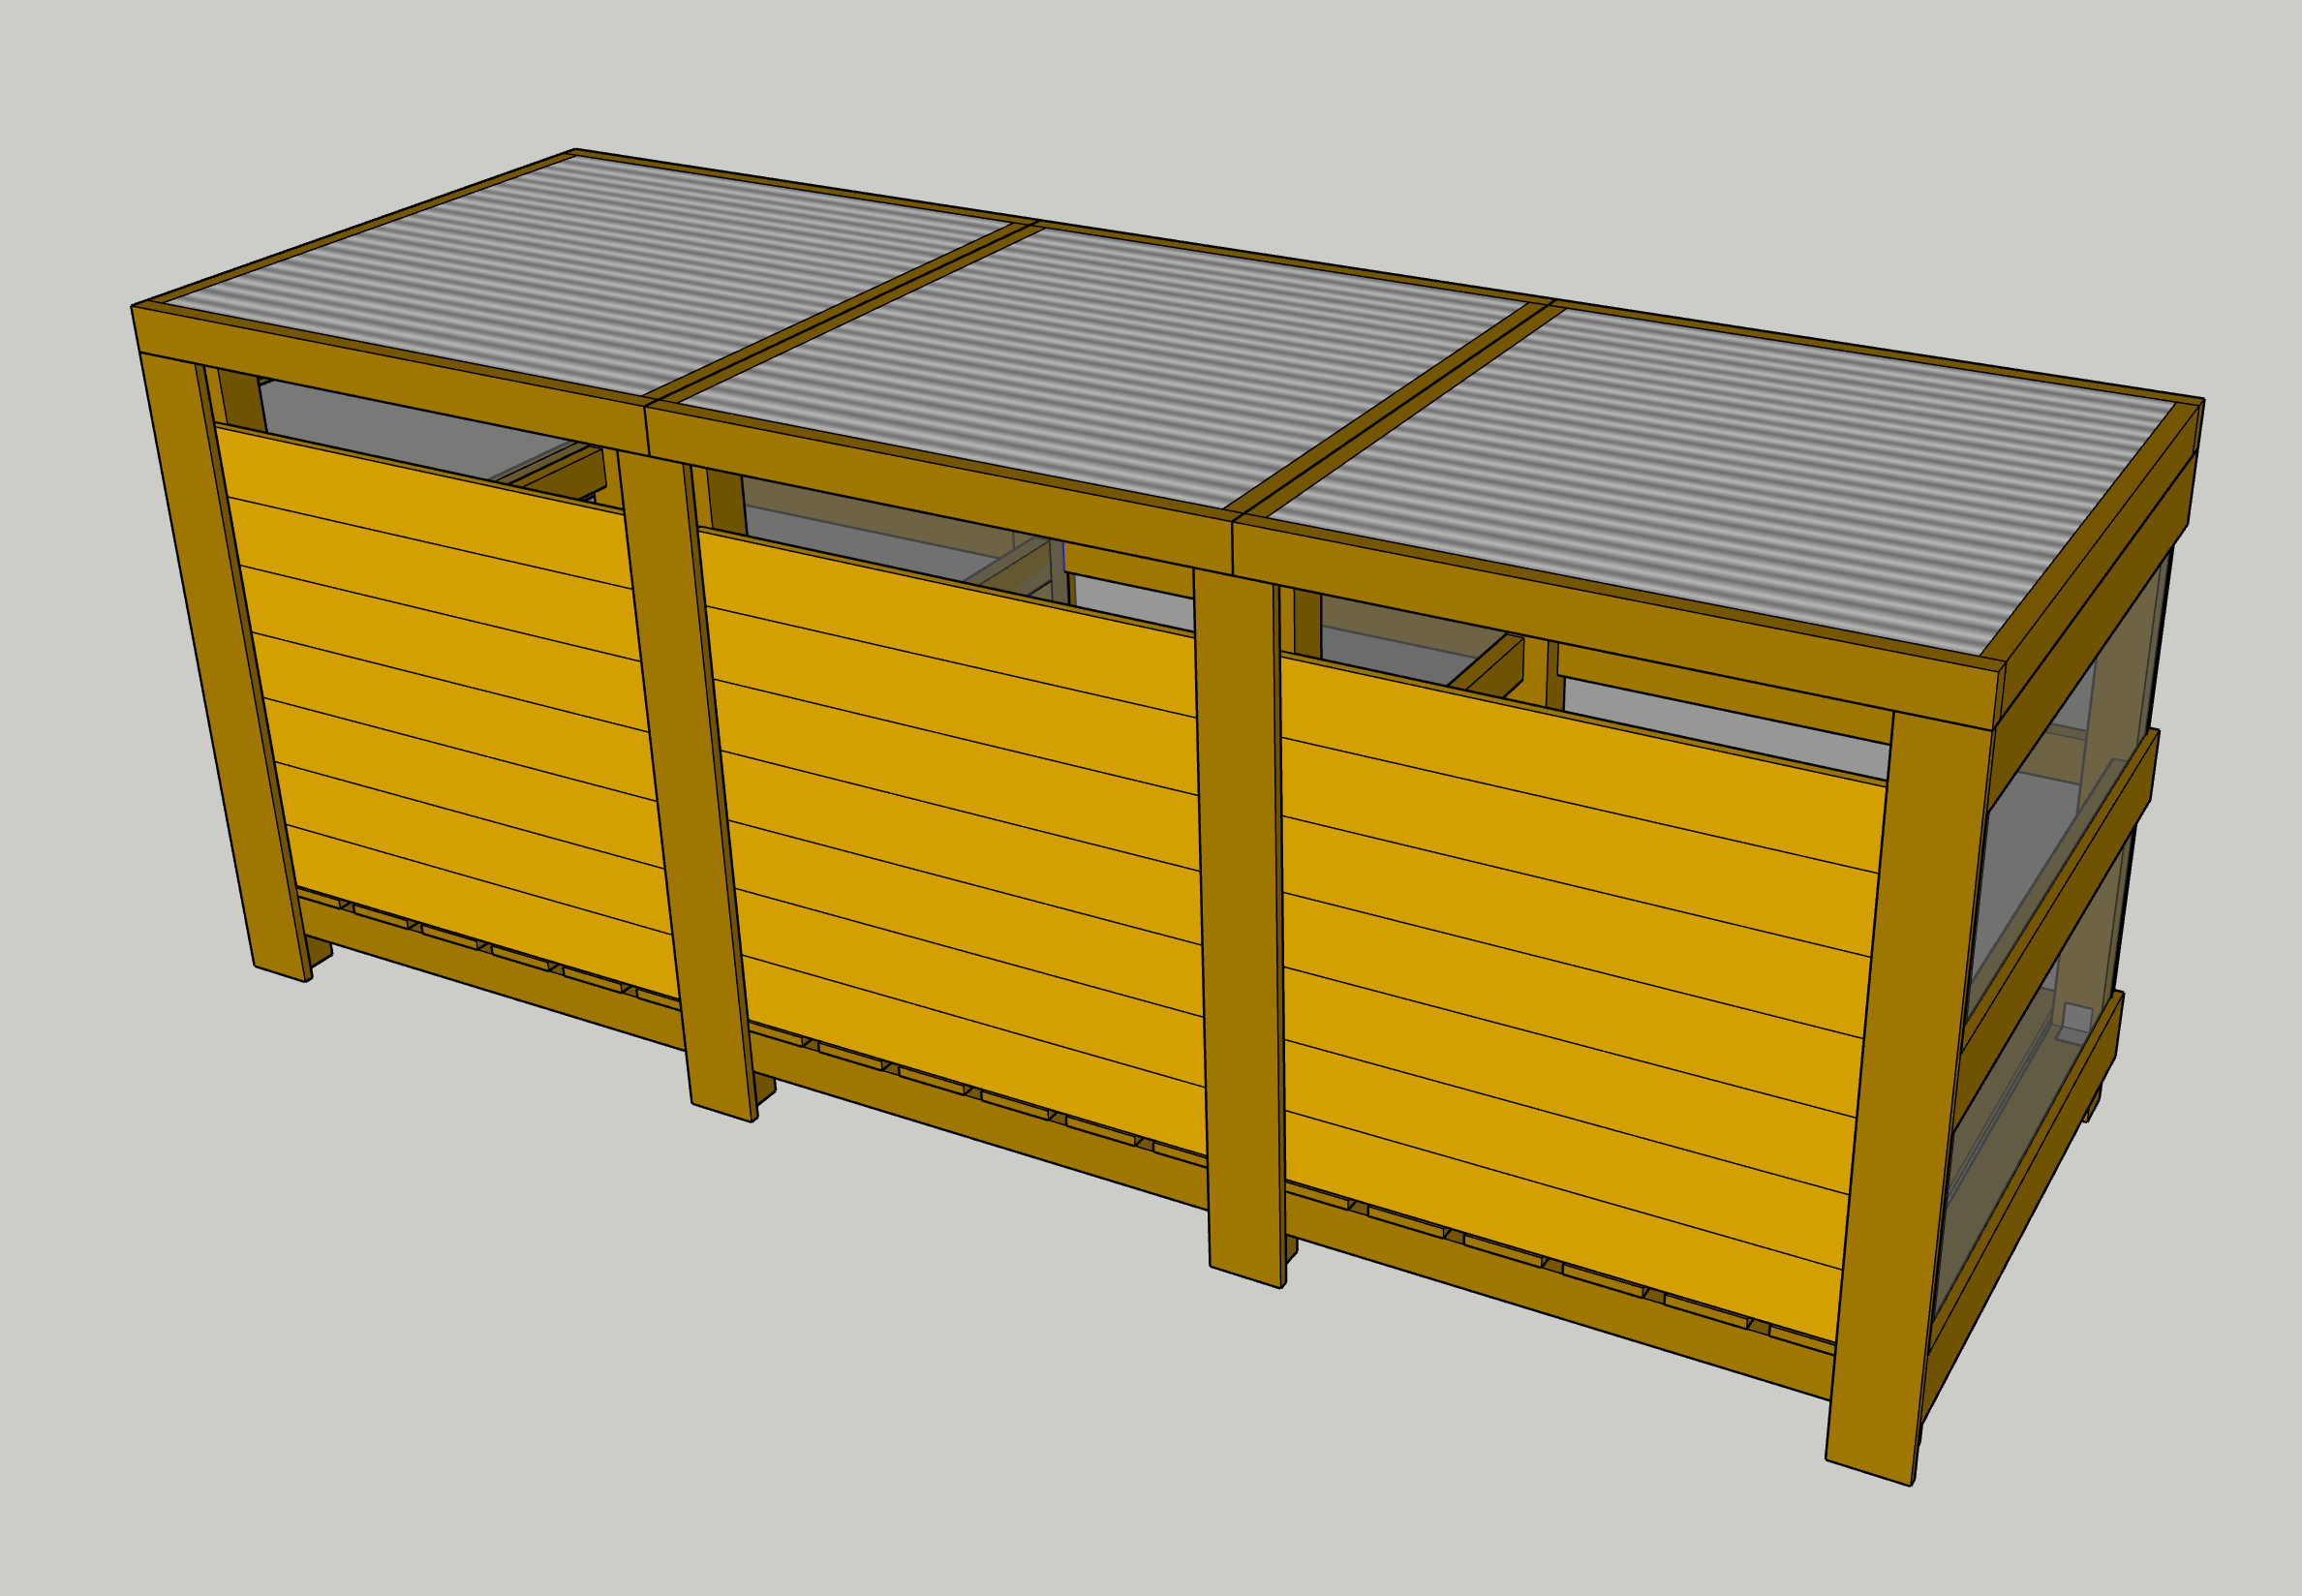
\includegraphics[width=.85\textwidth]{images/FrontPanels.png}
  \end{center}
\end{frame}

\begin{frame}
  \frametitle{Final Actual Construction}
  \begin{center}
  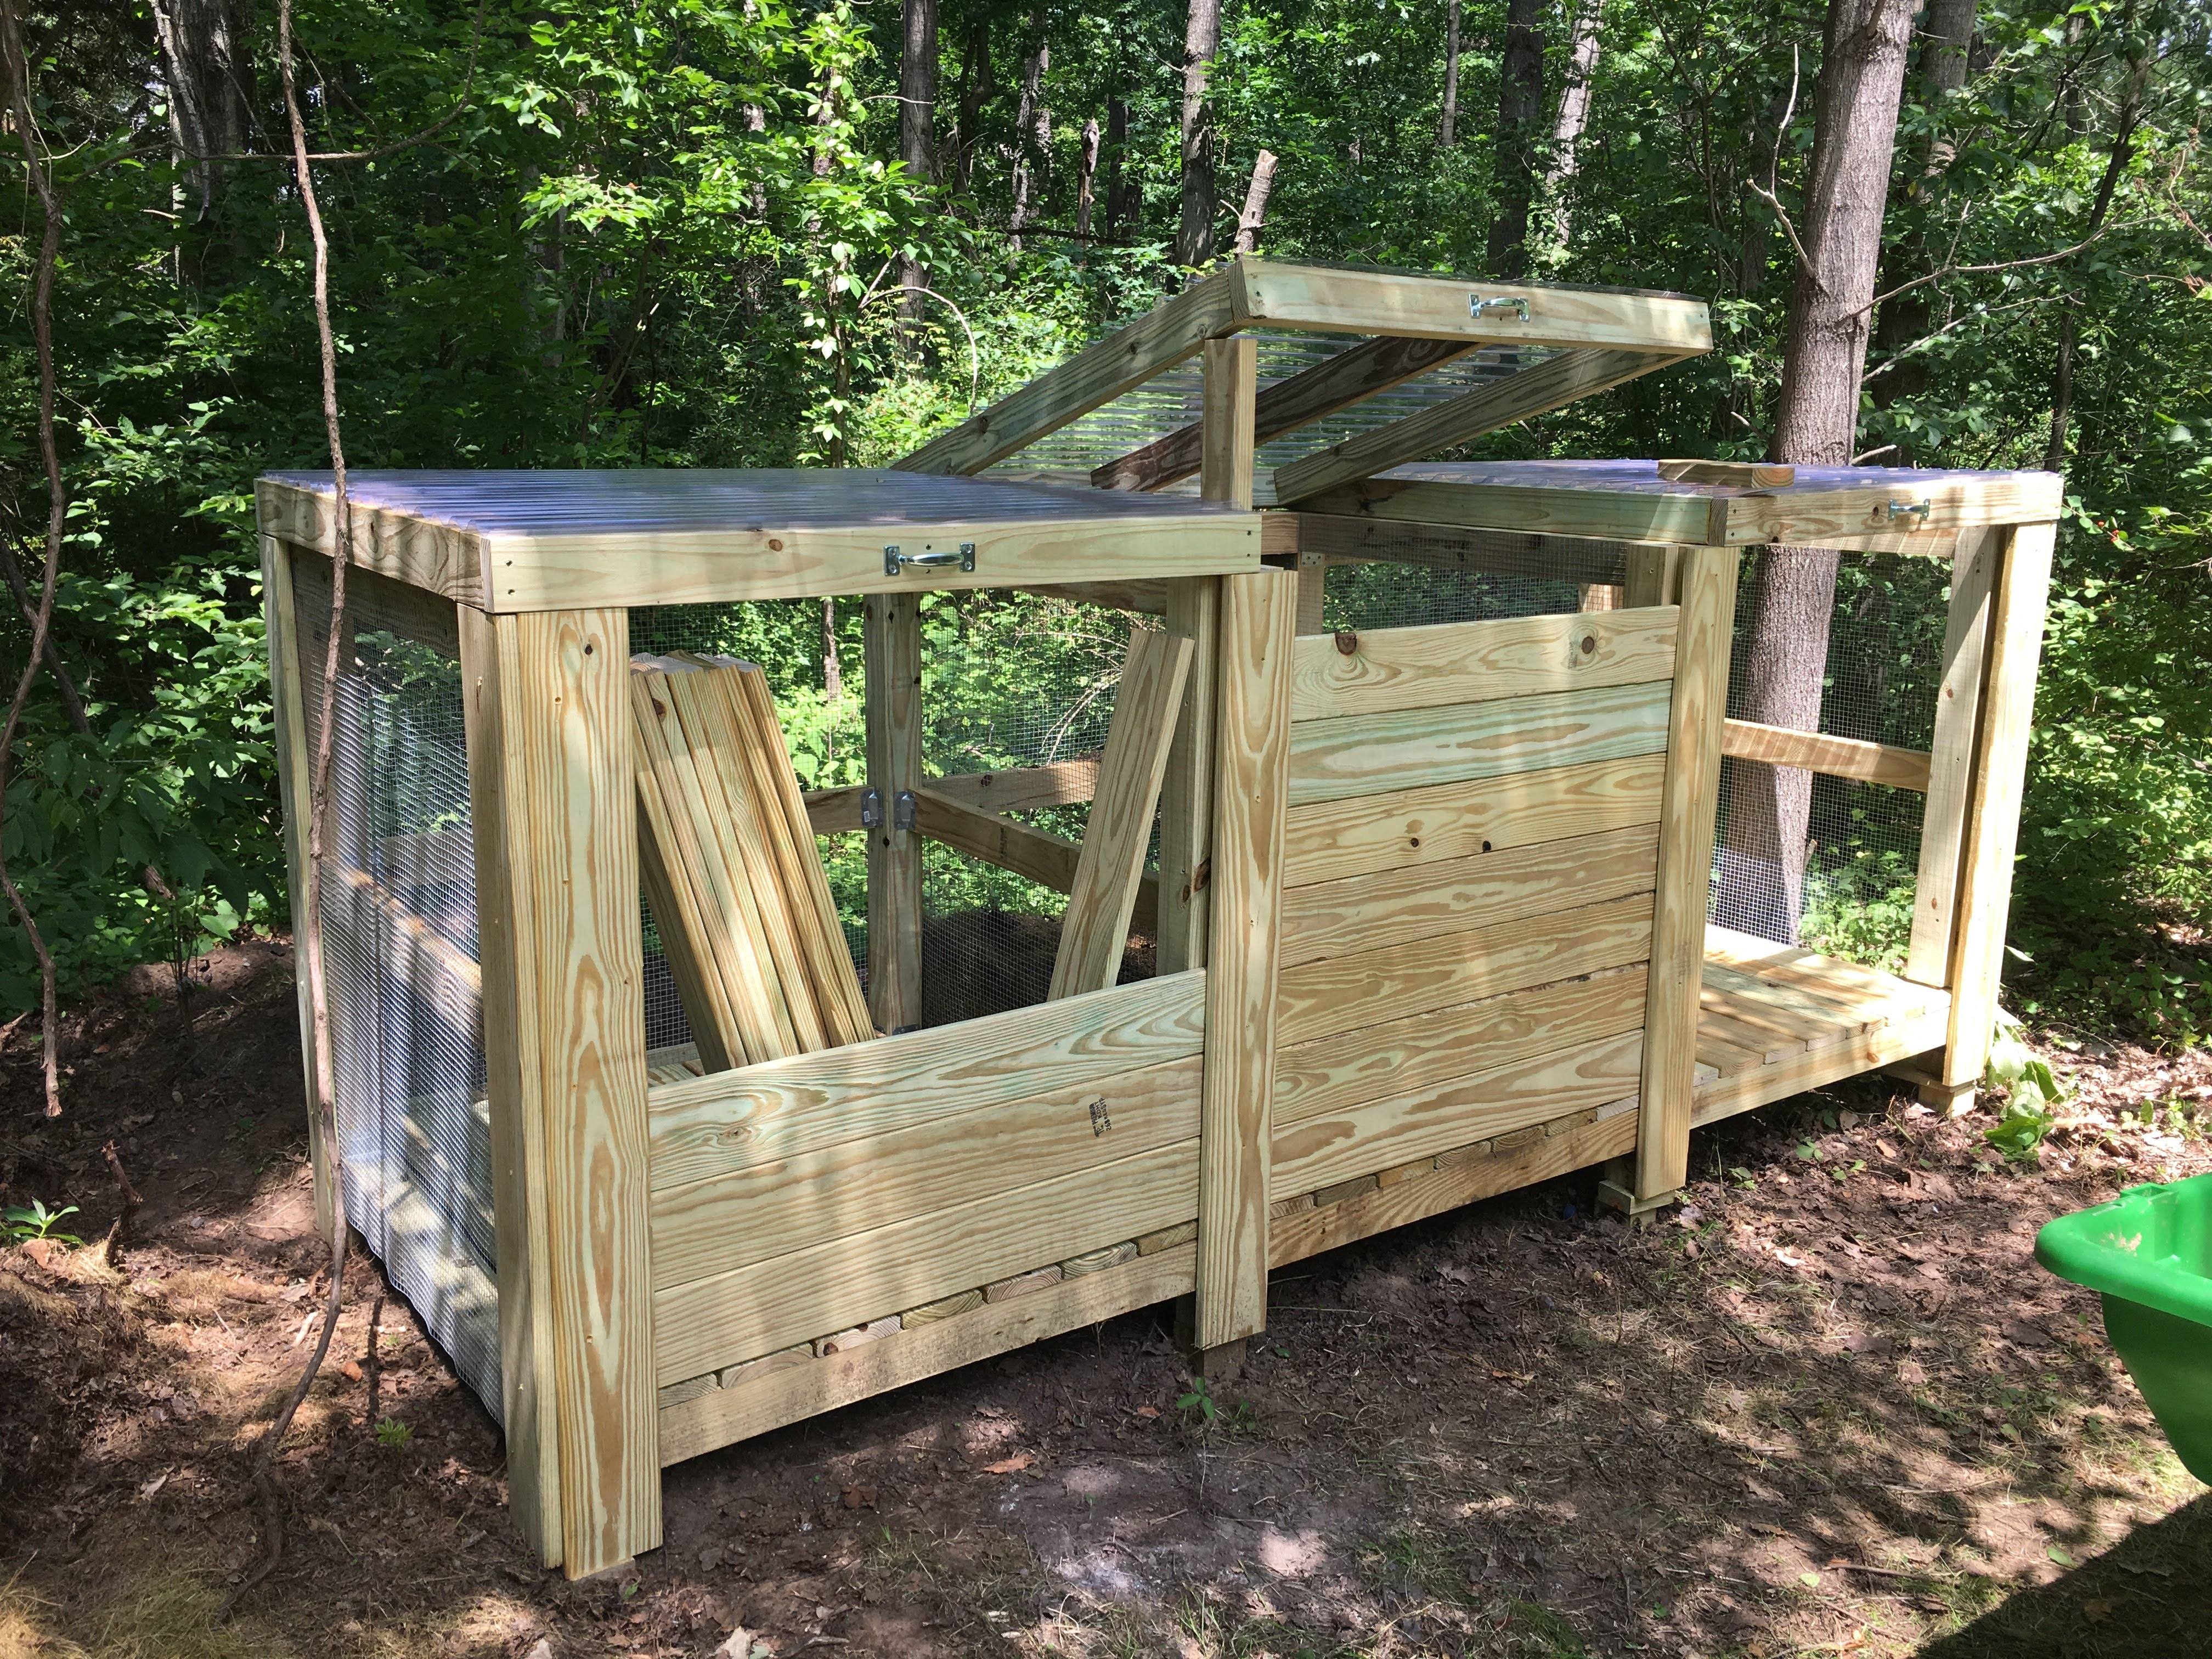
\includegraphics[width=.85\textwidth]{images/actual_finished.JPG}
  \end{center}
\end{frame}

\section{Recommendations}

\begin{frame}
  \frametitle{Possible Improvements}
  \begin{description}
  \item[Outside frame strengthening] The outside frames have tendency to lean outward as joints at three corners don't hold sufficiently. The struts go someway to minimizing the lean, but it'd be feasible to mount a bar across the top (it wouldn't really impact filling/emptying the bins at all)
  \item[Outside paneling] Full design should include paneling on the exterior over all the struts, clamping the wire grid securely between strut and panel. Otherwise staples take weight of compost pushing outward.
    \item[Lid foldback] May be beneficial for compost to not have lid always protecting from rain, a hinge with sufficient clearance at back would allow lid to be folded right over.
  \end{description}
\end{frame}

\end{document} 
